\documentclass[aspectratio=169]{beamer}

%% ─── Theme (Bruno: navy/red, Fira Sans, gray footer) ────────────────────────
\usetheme{Bruno}

%% frame titles: small and bold (overrides the theme's \Large)
\setbeamerfont{frametitle}{size=\normalsize, series=\bfseries}

%% ─── Packages ────────────────────────────────────────────────────────────────
\usepackage{pifont}
\usepackage{fontawesome5}
\usepackage{xcolor}
\usepackage{tikz}
\usetikzlibrary{arrows.meta, positioning, calc, shadows, shapes.callouts, overlay-beamer-styles, fit, patterns, fadings}
%% radial fading used to wash out the slide behind an overlaid callout
\tikzfading[name=softwash, inner color=transparent!0, outer color=transparent!100]
\usepackage{booktabs}
\usepackage{colortbl}
\usepackage{pgfplots}
\pgfplotsset{compat=1.18}
\usepackage{numprint}
\npthousandsep{,}  % 30,530,313 rather than numprint's default thin space
\usepackage{graphicx}
\usepackage{hyperref}

%% ─── Colors ──────────────────────────────────────────────────────────────────
\definecolor{tug}{RGB}{196,13,30}
\definecolor{tugb}{RGB}{60,100,200}
\definecolor{darkgreen}{RGB}{0,130,0}
\definecolor{mygreen}{RGB}{220,245,215}
\definecolor{myorange}{RGB}{255,230,210}
\definecolor{deepblue}{HTML}{1E40AF}
\definecolor{color4}{RGB}{255,165,0} % orange
\definecolor{cppblue}{HTML}{00599C} % the C++ logo blue




%% ─── Colored callout blocks ──────────────────────────────────────────────────
\setbeamercolor{block title example}{bg=darkgreen, fg=white}
\setbeamercolor{block body example}{bg=mygreen, fg=black}
\setbeamercolor{block title alerted}{bg=orange!80!black, fg=white}
\setbeamercolor{block body alerted}{bg=myorange, fg=black}

%% ─── Helpers ─────────────────────────────────────────────────────────────────
\newcommand{\hred}[1]{\textcolor{tug}{\textbf{#1}}}
\newcommand{\hgreen}[1]{\textcolor{darkgreen}{\textbf{#1}}}
\newcommand{\htug}[1]{\textcolor{tug}{\textbf{#1}}}
\newcommand{\hblue}[1]{\textcolor{tugb}{\textbf{#1}}}
\newcommand{\venue}[1]{\emph{\textbf{#1}}}
%% Every frame title is prefixed with the section/system it belongs to, so a
%% slide pulled up mid-question announces its own context.  Systems keep their
%% accent (tugb = CatDB, tug = ReSequel, darkgreen = ROLEX); the framing
%% sections (Introduction/Overview/Conclusion) use neutral gray.
%% #1 accent, #2 section or system, #3 title.
\newcommand{\apptitle}[3]{%
  \textcolor{#1}{#2}~\textcolor{black!30}{\textbar}~#3}
%% Conservative figure heights to fit in Bruno 16:9 slide
\newlength{\figH}    \setlength{\figH}{30mm}
\newlength{\figHfull}\setlength{\figHfull}{38mm}

%% ─── Compact item spacing ────────────────────────────────────────────────────
\setlength{\itemsep}{1pt}
\setlength{\parskip}{0pt}

%% ─── Metadata ────────────────────────────────────────────────────────────────
\title[LLM-assisted Data Systems for Efficient ML Pipeline Generation and Query Optimization]{LLM-assisted Data Systems for Efficient ML Pipeline Generation and Query Optimization}
\author{Saeed Fathollahzadeh}
\institute{Dissertation Defense\\[6pt]
August 21, 2026 }
\date{}

%%%%%%%%%%%%%%%%%%%%%%%%%%%%%%%%%%%%%%%%%%%%%%%%%%%%%%%%%%%%%%%%%%%%%%%%%%%
\begin{document}
%%%%%%%%%%%%%%%%%%%%%%%%%%%%%%%%%%%%%%%%%%%%%%%%%%%%%%%%%%%%%%%%%%%%%%%%%%%

%% ─── SLIDE 1: TITLE ──────────────────────────────────────────────────────────
\begin{frame}[plain,noframenumbering]
  \titlepage
\end{frame}

%% ─── SLIDE 2: HISTORICAL MOTIVATION ─────────────────────────────────────────
%% Scattered pile of landmark papers (full first pages).
%% Every page is drawn at a fixed WIDTH (in pt) and hangs as far down as it likes;
%% the \clip below cuts the whole pile at one bottom line, so the lower part of
%% each page is simply hidden.  Move a paper by editing its (x,y) pair: x = its
%% place along the timeline, y = how high it sits (anchor = top-left corner).
\begin{frame}{\apptitle{black!60}{Introduction}{Automating Data Systems: A Mainstay for Decades!}}
\vspace{4mm}
\centering
\resizebox{\linewidth}{!}{%
\begin{tikzpicture}[
  pg/.style={draw=tug, fill=white, line width=0.4pt, inner sep=0, anchor=north west,
    drop shadow={shadow xshift=1.5pt, shadow yshift=-1.5pt, fill=tug!50}},
      pgml/.style={draw=blue!55, fill=white, line width=0.4pt, inner sep=0, anchor=north west,
    drop shadow={shadow xshift=1.5pt, shadow yshift=-1.5pt, fill=blue!30}},
  plbl/.style={anchor=north, align=center, font=\scriptsize, text width=3.0cm}
]
  %% ── the pile: clipped at y = -2.05, i.e. the bottom of every page is hidden ─
  \begin{scope}
    %% SQL thread
    \node[pg, rotate=0] at (-0.30, 0) {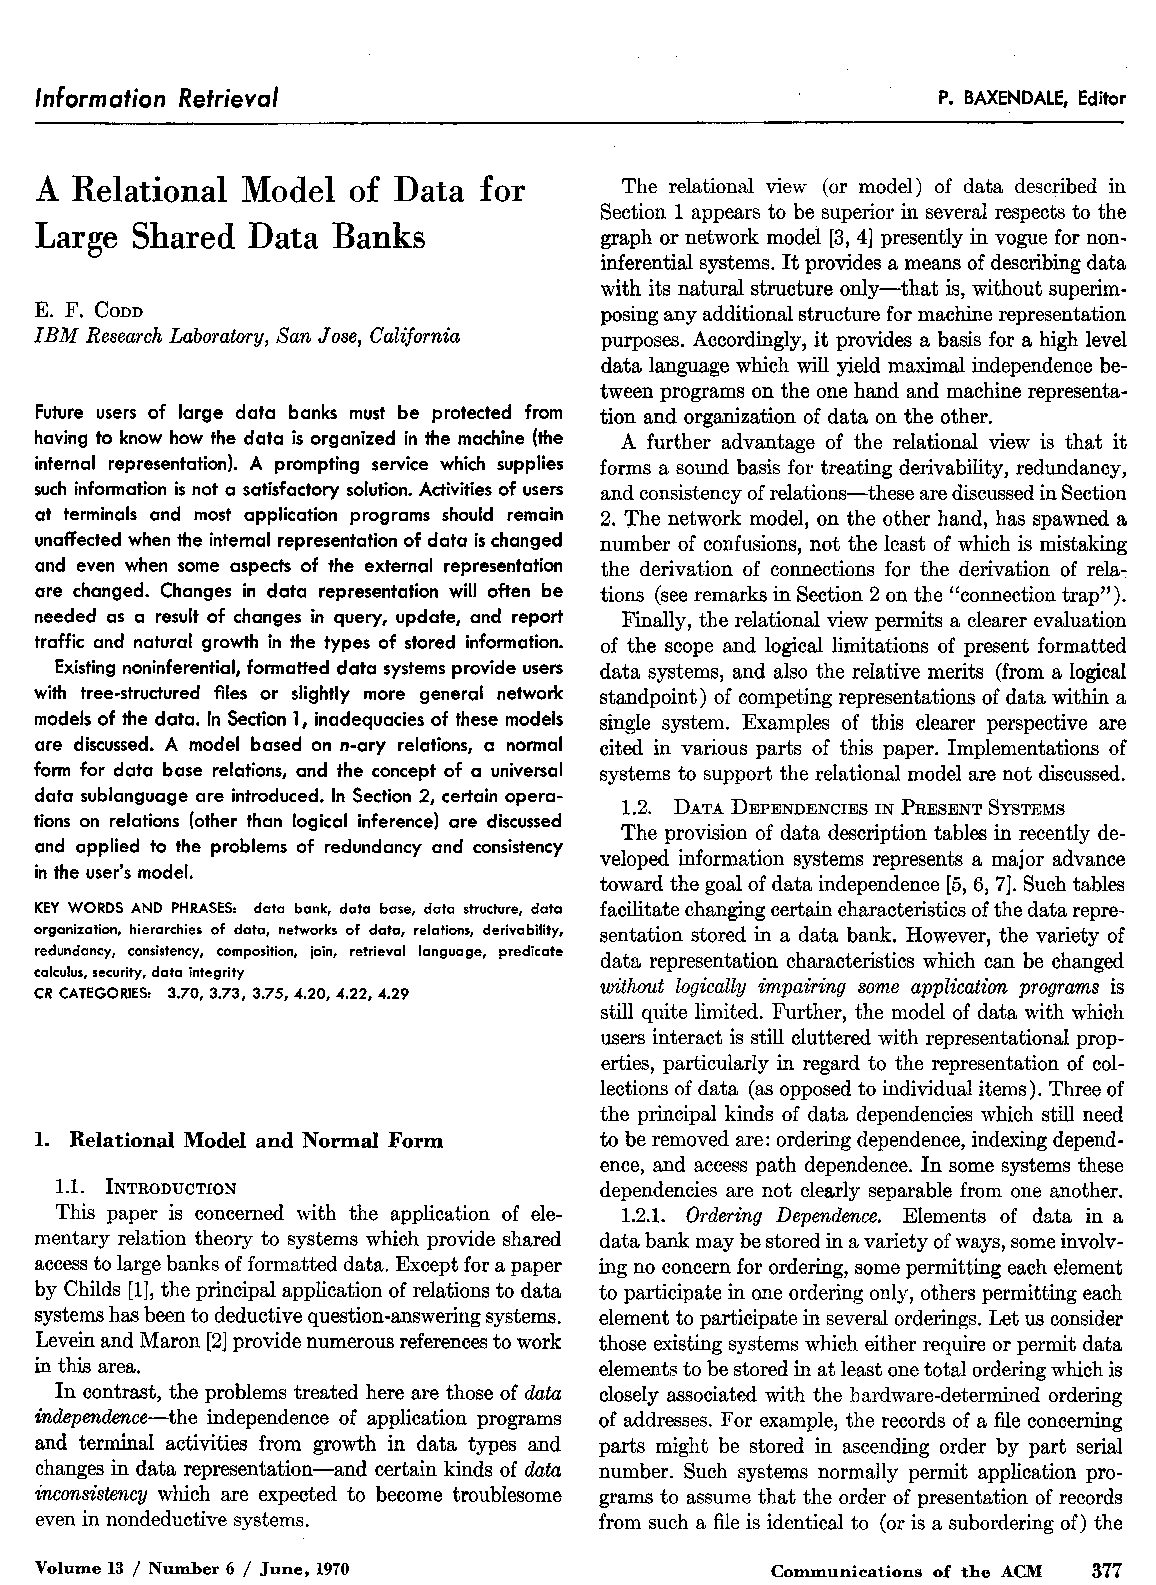
\includegraphics[width=100pt]{fig/Codd1970-p1.pdf}};
      \node[pgml] at (4.35,0) {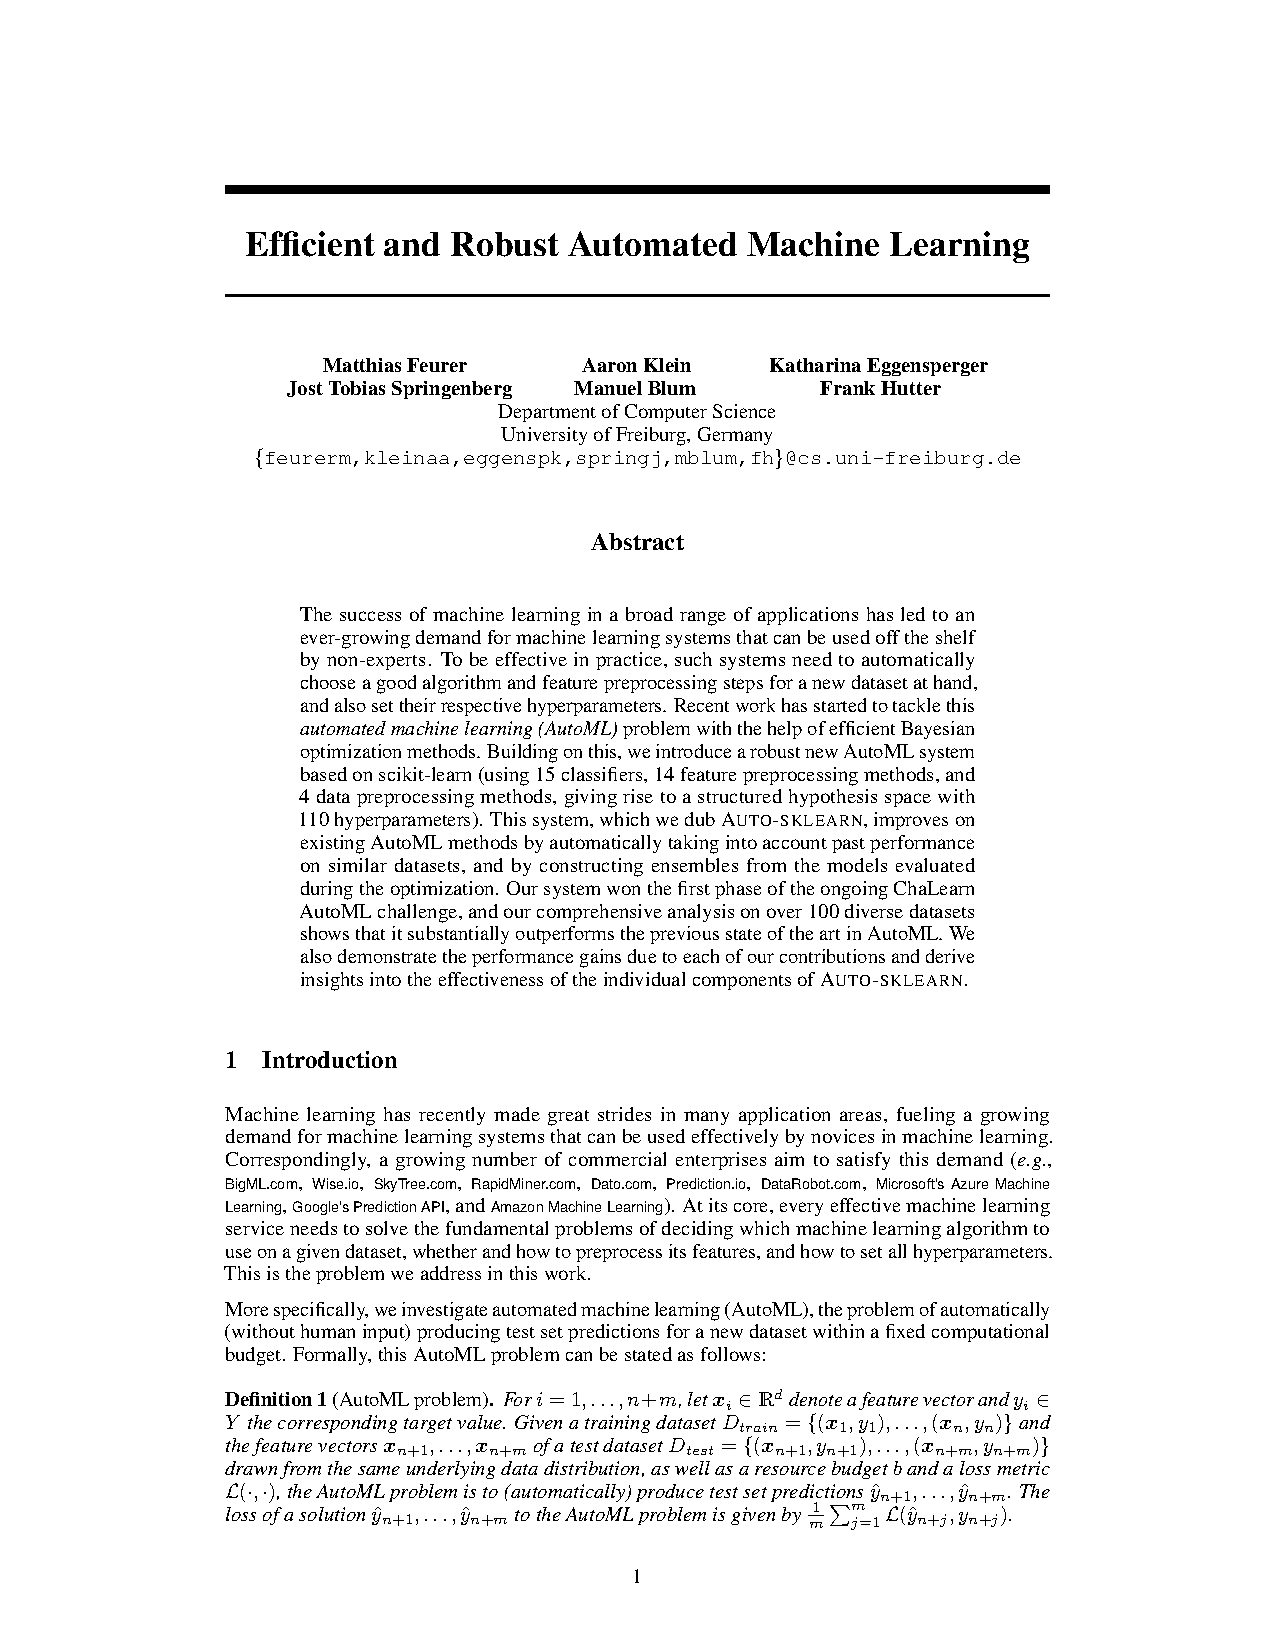
\includegraphics[width=100pt]{fig/AutoSklearn2015-p1.pdf}};

    \node[pg, rotate=0] at (1.40,-0.40) {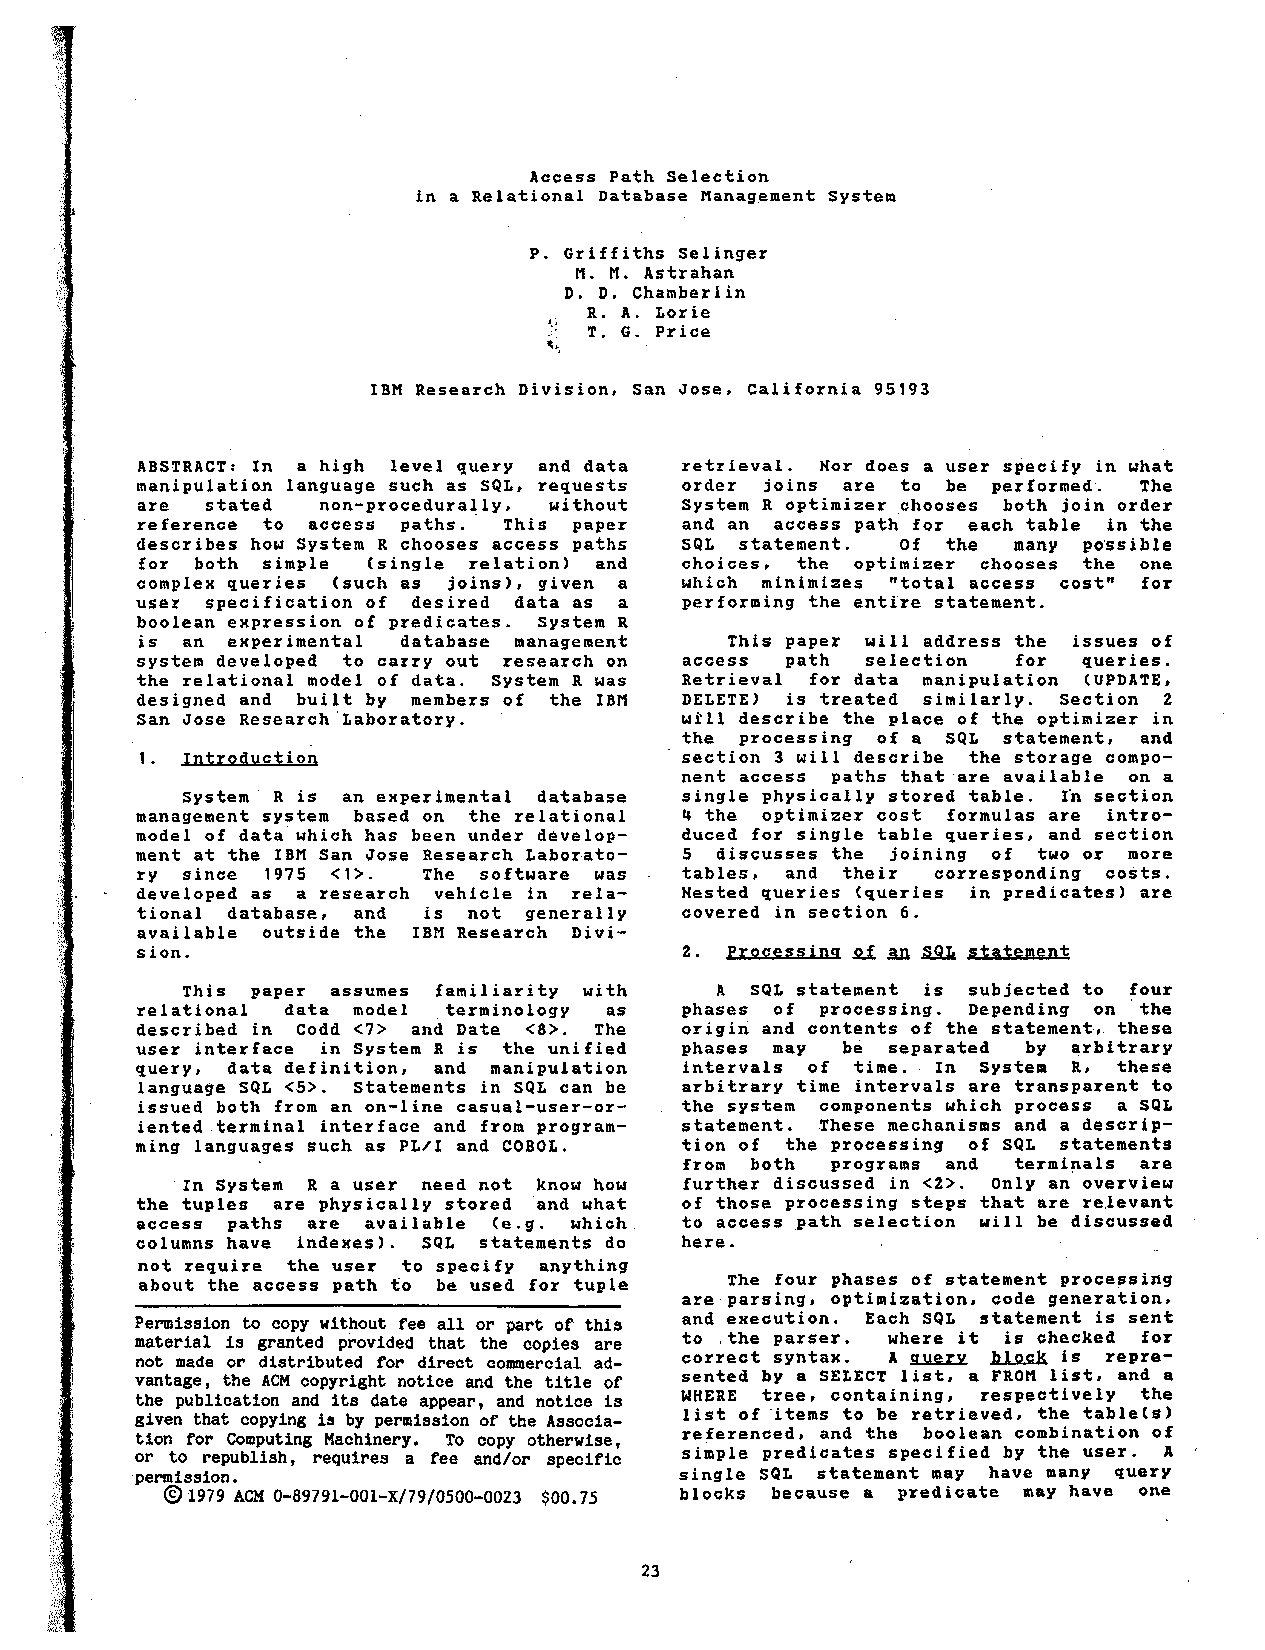
\includegraphics[width=100pt]{fig/Selinger1979-p1.pdf}};
    \node[pg, rotate=0] at (0.40, -1.30) {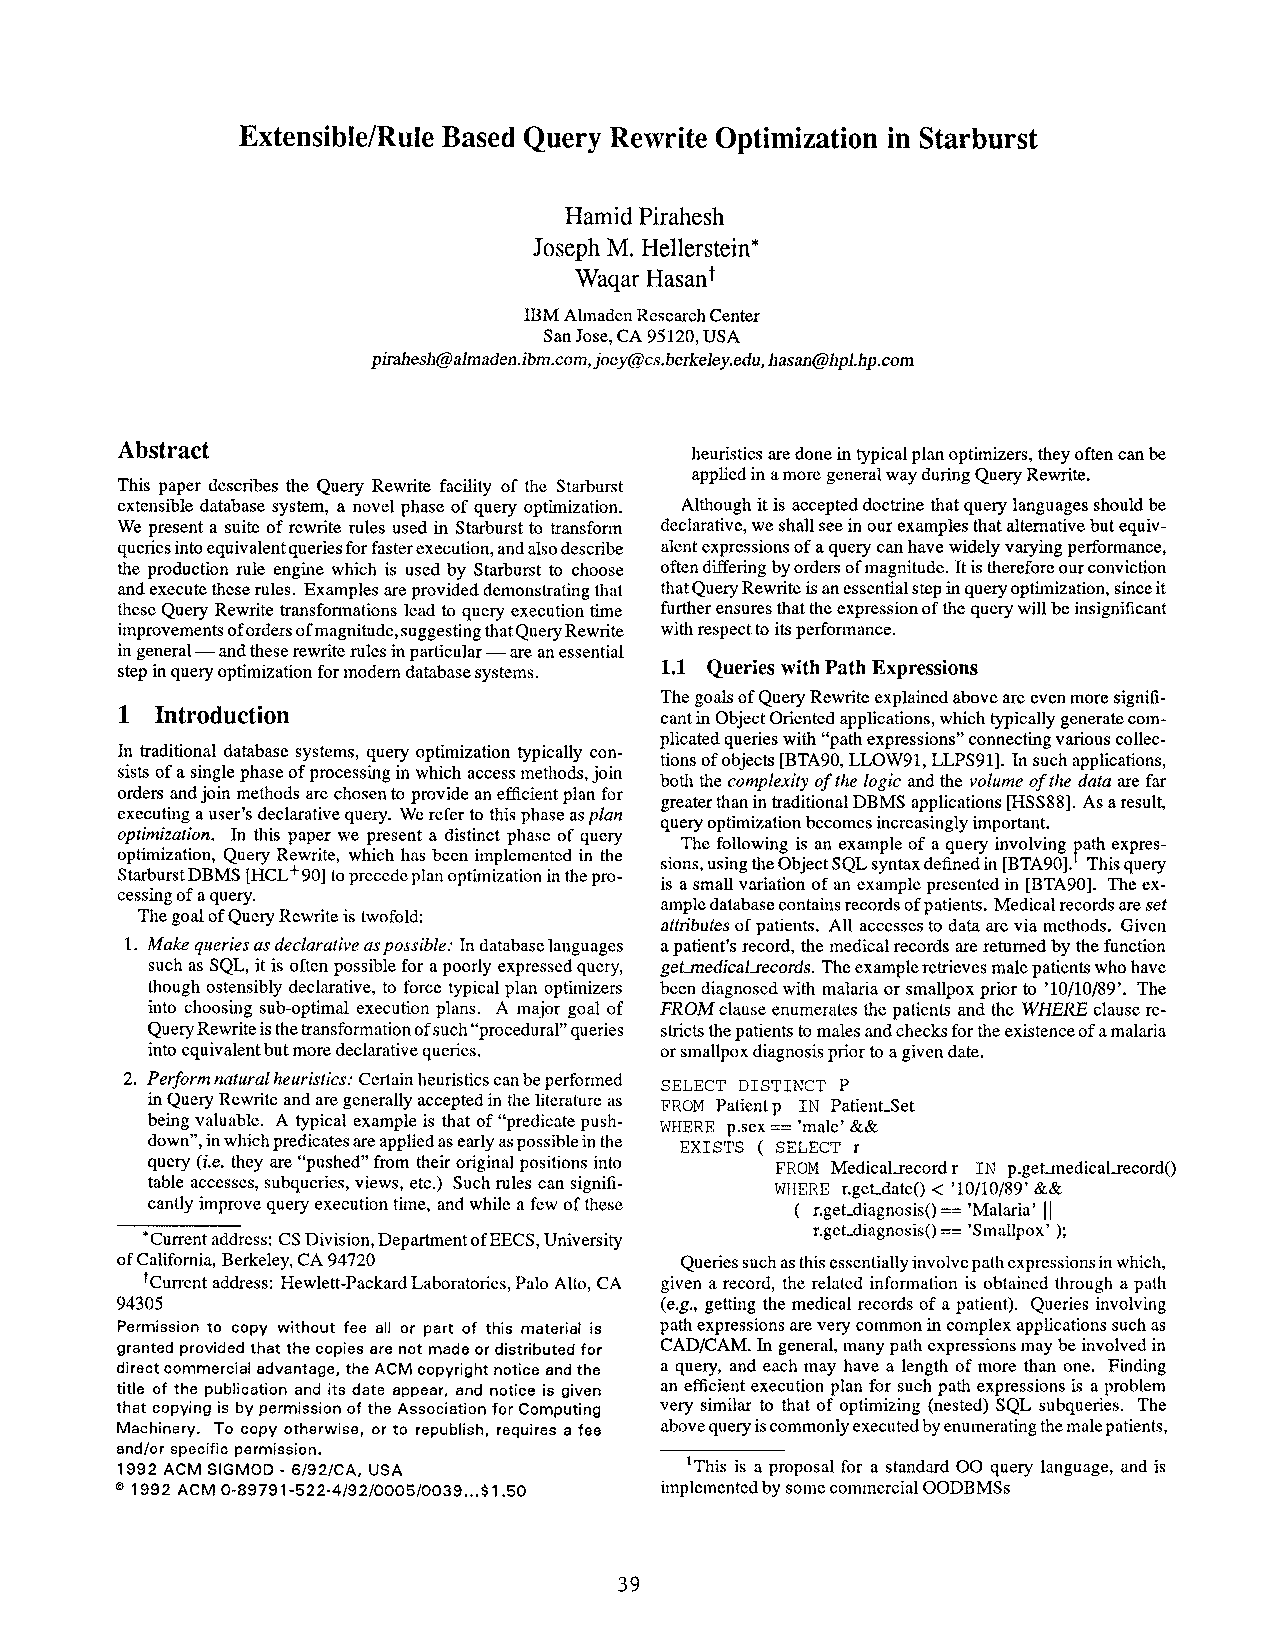
\includegraphics[width=100pt]{fig/Starburst1992-p1.pdf}};

    \node[pgml] at (5.20, -1.35) {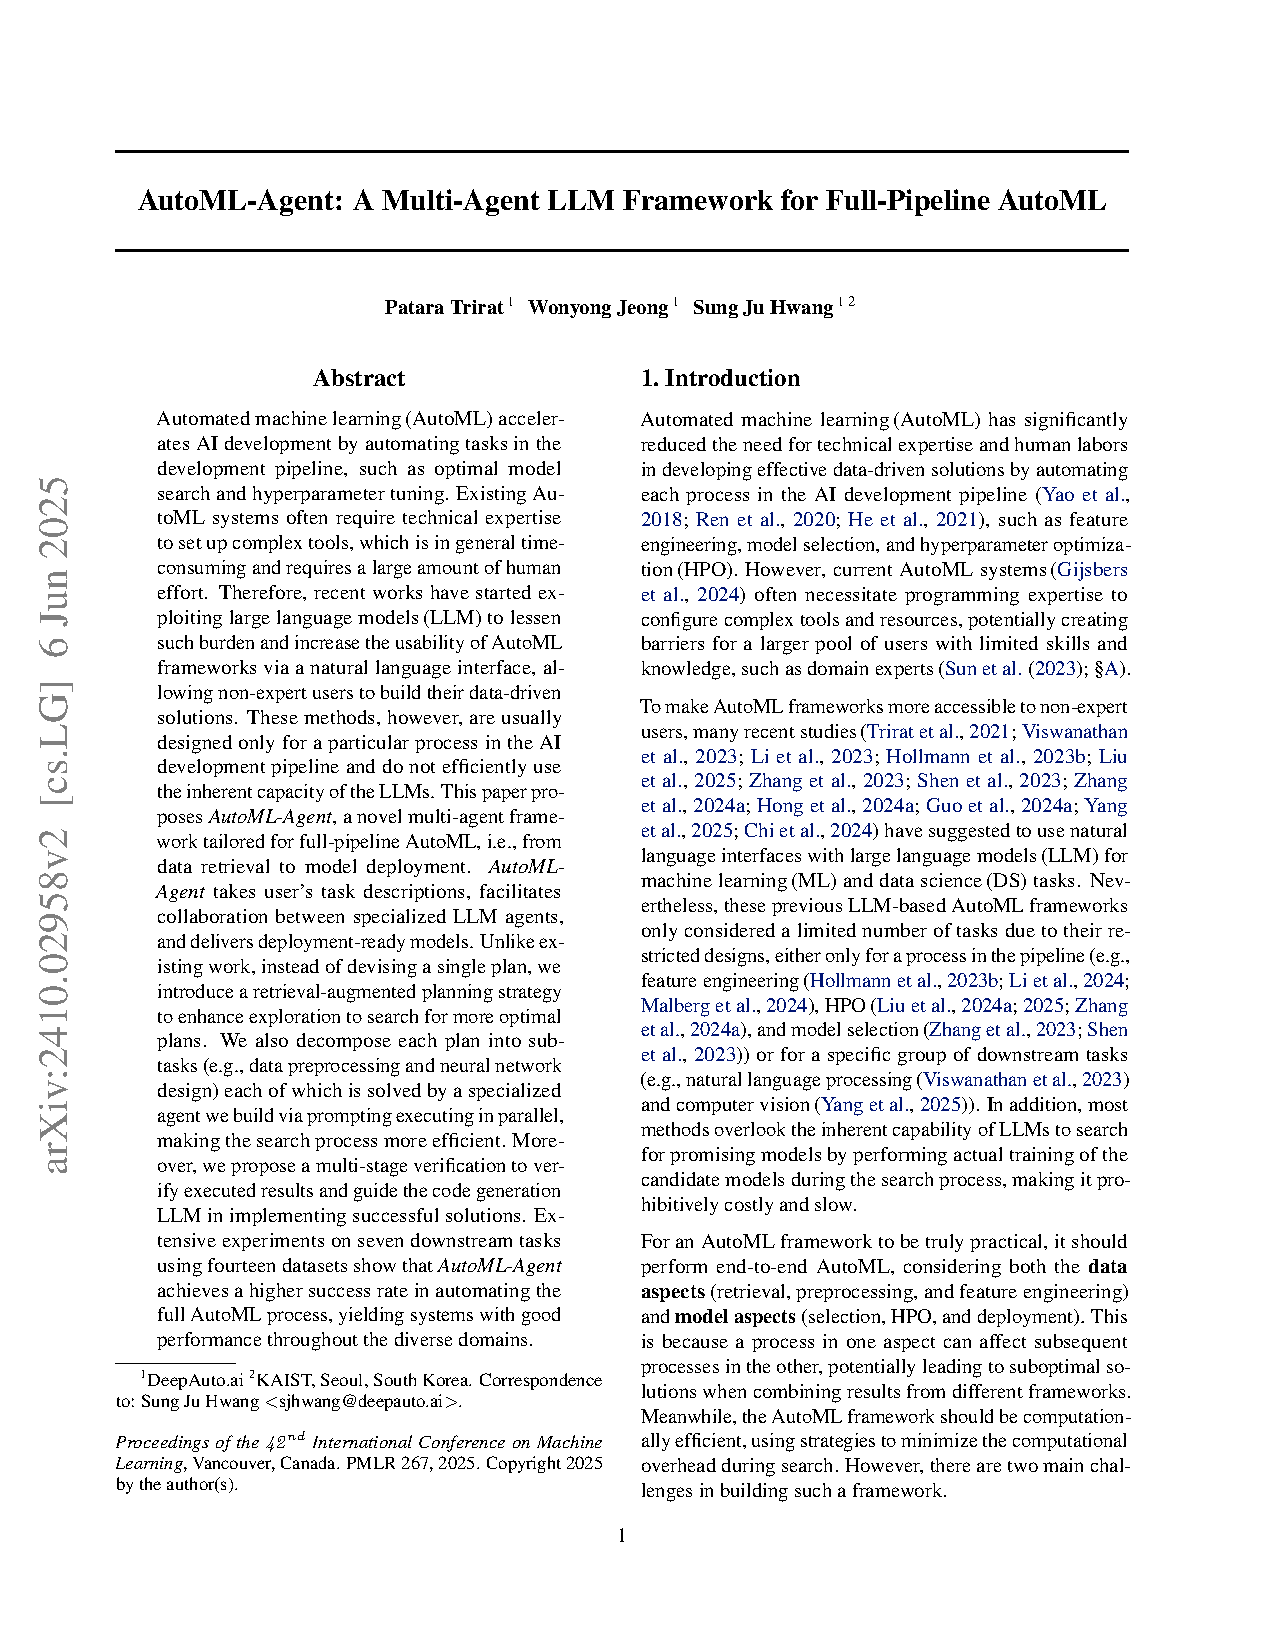
\includegraphics[width=90pt]{fig/AutoMLAgent2025-p1.pdf}};
   
  \end{scope}

\end{tikzpicture}}

%% takeaway revealed on a click, laid over the pile so the figure is untouched
\only<2->{%
\begin{tikzpicture}[remember picture, overlay]
  \node[anchor=center, text width=0.80\paperwidth, align=center,
        rounded corners=2.5pt, fill=darkgreen!14, draw=darkgreen!55,
        line width=0.6pt, inner sep=3.5mm, font=\small]
    at ($(current page.center)+(0,-14mm)$)
    {Fifty years of work, one recurring idea: \hgreen{take a decision that
     requires an expert}, and let the \hgreen{system} make it instead.};
\end{tikzpicture}}
\end{frame}

%% ─── ECOSYSTEM SLIDES ───────────────────────────────────────────────────────
%% Logo walls in the style of the sample deck.  Logos live in fig/logos/;
%% each one is scaled into a fixed-size cell so rows never overflow.
%% Systems without a public logo are drawn as text chips.
\newlength{\logoH}\setlength{\logoH}{9mm}
%% every logo sits in a cell of the same width *and* height, so a row is exactly
%% \logoCellH tall no matter how flat or tall the individual artwork is -- that
%% keeps the two ecosystem slides on the same baselines when flipping between
%% them.  \logoCellH must stay >= the largest per-logo height used below, and
%% six cells (the widest row) must still fit inside \textwidth -- a row that
%% overflows the text block also drags the whole slide body downwards.
\newlength{\logoCellH}\setlength{\logoCellH}{11.5mm}
\newlength{\logoCellW}\setlength{\logoCellW}{23mm}
%% \logopic[<height>]{<file>} -- optional height for square icons
\newcommand{\logopic}[2][\logoH]{%
  \makebox[\logoCellW][c]{%
    \parbox[c][\logoCellH][c]{\dimexpr\logoCellW-2mm\relax}{\centering
      \includegraphics[height=#1, width=\dimexpr\logoCellW-2mm\relax,
                       keepaspectratio]{fig/logos/#2}}}}
%% Text chips drawn like a CPU package: tugb body, three pins per side and the
%% little pin-1 dot on the left.  Pins hang outside the node, so the trailing
%% \hspace between chips already leaves room for them.
\tikzset{
  %% text height/depth are pinned so a chip is the same height (and sits on the
  %% same baseline) whether or not its label has ascenders or descenders --
  %% "TPOT" and "AutoGluon" must not draw differently sized packages.
  chipbody/.style={rounded corners=1.5pt, draw=tugb!75, line width=0.5pt,
                   fill=tugb!12, inner xsep=5pt, inner ysep=2.5pt,
                   text height=1.5ex, text depth=0.35ex,
                   text=tugb!80!black, font=\scriptsize},
  chippin/.style={draw=tugb!75, line width=0.9pt, line cap=round},
}
\newcommand{\chip}[1]{%
  \begin{tikzpicture}[baseline=-3pt]
    \node[chipbody] (c) {#1};
    %% pins: three evenly spaced stubs on each vertical edge
    \foreach \pinpos in {0.25, 0.5, 0.75}{%
      \draw[chippin] ($(c.north west)!\pinpos!(c.south west)$) -- ++(-1.8pt,0);
      \draw[chippin] ($(c.north east)!\pinpos!(c.south east)$) -- ++( 1.8pt,0);
    }
    %% pin-1 marker, kept inside the 5pt inner xsep so it never touches the text
    \fill[tugb!75] ($(c.west)+(2.5pt,0)$) circle (0.8pt);
  \end{tikzpicture}}

%% ─── SLIDE: ML ECOSYSTEM ─────────────────────────────────────────────────────
\begin{frame}[t]{\apptitle{black!60}{Introduction}{The Result? An Ecosystem of Libraries --- and Users}}
\vspace{2mm}
\begin{center}
  \logopic{sklearn.png}\logopic{pandas.png}\logopic{numpy.png}\logopic{scipy.png}\logopic{xgboost.png}\\[4mm]
  \logopic{pytorch.png}\logopic{tensorflow.png}\logopic{keras.png}\logopic{huggingface.png}\\[4mm]

  {\footnotesize\textcolor{gray}{+ AutoML and LLM-based pipeline builders}}\\[2mm]
  \chip{auto-sklearn}\hspace{2mm}\chip{AutoGluon}\hspace{2mm}\chip{TPOT}\hspace{1mm}%
  \chip{H2O AutoML}\hspace{2mm}\chip{CAAFE}\hspace{2mm}\chip{AIDE}\hspace{2mm}\chip{AutoML-Agent}
\end{center}
\vspace{2mm}
\begin{alertblock}{}
  \centering
  Thousands of building blocks --- but \hred{choosing, cleaning, configuring and gluing}
  them is still \textbf{manual expert work}
\end{alertblock}
\end{frame}

%% ─── SLIDE: DBMS ECOSYSTEM ───────────────────────────────────────────────────
\begin{frame}[t]{\apptitle{black!60}{Introduction}{The Result? An Ecosystem of Engines and Optimizers}}
\vspace{2mm}
\begin{center}
  \logopic{postgres.png}\logopic{mysql.png}\logopic{sqlite.png}\logopic{duckdb.png}\logopic{oracle.png}\logopic[11mm]{gaussdb.png}\\[4mm]
  \logopic{spark.png}\logopic{clickhouse.png}\logopic{snowflake.png}\logopic{trino.png}\logopic{databricks.png}\\[4mm]

  {\footnotesize\textcolor{gray}{+ decades of rewrite rules and optimizer frameworks}}\\[2mm]
  \chip{System R}\hspace{2mm}\chip{Starburst}\hspace{2mm}\chip{Volcano/Cascades}\hspace{1mm}%
  \chip{Apache Calcite}\hspace{2mm}\chip{LearnedRewrite}\hspace{2mm}\chip{R-Bot}
\end{center}
\vspace{2mm}
\begin{alertblock}{}
  \centering
  Same data, same semantics --- runtime still varies by \hred{orders of magnitude}
  with how the query is \textbf{written}
\end{alertblock}
\end{frame}



\begin{frame}{\apptitle{black!60}{Introduction}{Example 1 --- Generate Pipelines for Unseen Datasets}}

  \tiny
  \begin{tikzpicture}
    \node[fill=white,inner sep=0, text=black, xshift=-10pt, line width=0.5pt]  (ds) {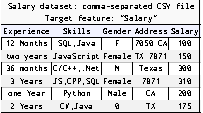
\includegraphics[scale=1.2] {fig/fig_salary_ds.pdf}};

    \node[visible on=<2->, draw=lightgray,fill=tugb!10,inner sep=1mm, text=black, right=of ds, xshift=2pt]  (description) {
      \shortstack[l]{\textbf{Generate a data science pipeline.}\\[3pt]
      \textcolor{black}{Experience} $\to$ \textcolor{tug}{string}, \texttt{100\%} distinct\\
      \textcolor{black}{Skills}$\to$ \textcolor{tug}{string}, \texttt{100\%} distinct\\
      \textcolor{black}{Gender}$\to$ \textcolor{tug}{categorical}, \texttt{60\%} distinct\\
      \textcolor{black}{Address}$\to$ \textcolor{tug}{string}, \texttt{100\%} distinct\\[3pt]
      \textbf{Build an ensemble model to forecast \textcolor{blue}{salary}.}
      }
      };
    
    \draw[visible on=<2->, -{Latex[scale=.6]}, line width=0.65pt, tugb] ($(description.north west)+(-32pt,-6pt)$) -- ($(description.north west)+(3pt,-6pt)$);  

    \draw[visible on=<2->, -{Latex[scale=.6]}, line width=0.65pt, tugb] ($(description.south west)+(-32pt,6pt)$) -- ($(description.south west)+(3pt,6pt)$);  

    \draw[visible on=<2->, {Latex[scale=.6]}-{Latex[scale=.6]}, line width=0.65pt, tugb] ($(description.north west)+(3pt,-18pt)$) -- ($(description.north west)+(-3pt,-18pt)$) -- ($(description.south west)+(-3pt,18pt)$) -- ($(description.south west)+(3pt,18pt)$); 

    \draw[visible on=<2->, -, line width=0.65pt, tugb] ($(description.west)+(-32pt,0pt)$) -- ($(description.west)+(-3pt,0pt)$);  

    \node[visible on=<2->, fill=none,inner sep=0, text=tugb] at ($(description.north west)+(-20pt,0pt)$)  (task) {Task};
    \node[visible on=<2->, fill=none,inner sep=0, text=tugb] at ($(description.south west)+(-15pt,0pt)$)  (prompt) {Prompt};
    \node[visible on=<2->, fill=none,inner sep=0, text=tugb] at ($(description.west)+(-18pt,4pt)$)  (metadata) {Metadata};

    %%%%%%%%%%%%%%%%%%%%%%%%%%%%
    \node[visible on=<2->, fill=white,inner sep=0,xshift=-10pt, right=of description ]  (llm) {
\includegraphics[scale=1.2] {fig/fig_LLM.pdf}};
    \draw[visible on=<2->, -{Latex[scale=.7]}, line width=0.8pt, tugb] (description) -- (llm);

    \node[visible on=<3->, draw=lightgray,fill=lightgray!40,inner sep=1.5mm,xshift=-10pt, right=of llm ]  (pipeline) {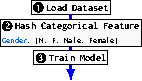
\includegraphics[scale=1.2] {fig/fig_metadata_pipDAG.pdf}};
    \draw[visible on=<3->, -{Latex[scale=.7]}, line width=0.8pt, tugb] (llm) -- (pipeline);   
    
    %%%%%%%%%%%%%%%%%%%%%%%%%%%%%
    \node[visible on=<4->, draw=none,fill=none,inner sep=0,xshift=0pt, below=of ds ]  (automl) {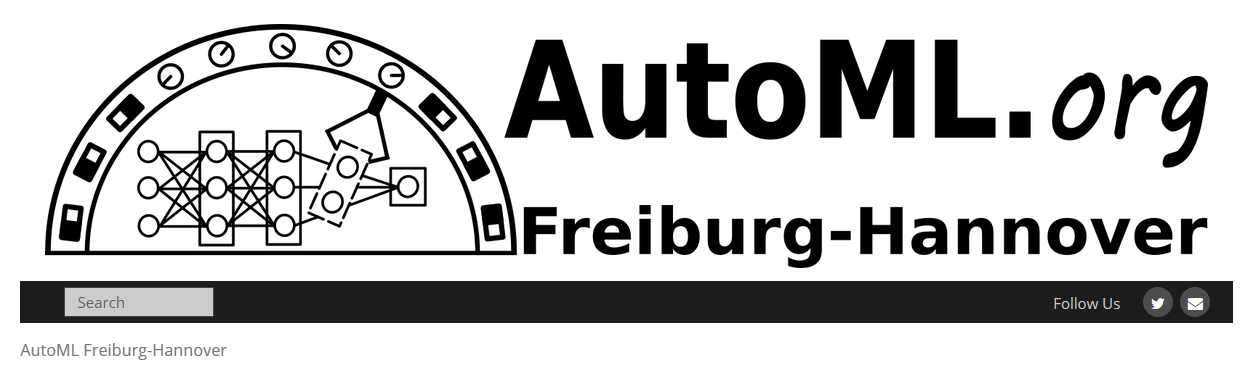
\includegraphics[scale=0.08] {fig/automl.png}};
     \draw[visible on=<4->, -{Latex[scale=.7]}, line width=0.8pt, black] (ds) -- (automl); 

    %%%%%%%%%%%%%%%%%%%%%%%%%%%%%

    \node[visible on=<5->, fill=darkgreen!50,inner sep=0, xshift=200pt, yshift=-20pt, line width=0.5pt, right=of automl, minimum width=25pt, minimum height=16.8pt]  (automlperformance) {};
    \node[visible on=<5->, fill=darkgreen,inner sep=0, xshift=-30pt, yshift=1.4pt, line width=0.5pt, right=of automlperformance, minimum width=25pt, minimum height=19.6pt, node distance=0]  (llmperformance) {};

    \draw[visible on=<5->, {Latex[scale=.6]}-{Latex[scale=.6]}, line width=0.65pt, gray] ($(automlperformance.north west)+(-5pt,50pt)$) |- ($(llmperformance.south east)+(10pt,0pt)$); 
    
    \node[visible on=<5->, fill=none,inner sep=0, xshift=0pt, yshift=-26pt, above=of automlperformance, text=black]  {32.6\%};
    \node[visible on=<5->, fill=none,inner sep=0, xshift=0pt, yshift=-26pt, above=of llmperformance, text=black]  {39.2\%};
    \node[visible on=<5->, fill=none,inner sep=0, xshift=13pt, yshift=40pt, left=of automlperformance, text=black, rotate=90] (acc) {Accuracy [\%]};

    \node[visible on=<5->, fill=none,inner sep=0, xshift=0pt, yshift=26pt, below=of automlperformance, text=black]  {AutoML};
    \node[visible on=<5->, fill=none,inner sep=0, xshift=0pt, yshift=26pt, below=of llmperformance, text=black]  {LLM};

    \draw[visible on=<5->, -{Latex[scale=.7]}, line width=0.8pt, lightgray] (automl) -- ($(acc)+(-20pt,0pt)$); 
  \end{tikzpicture}

\end{frame}


%% ─── Example 2 ──────────────────────────────────────────────────────
\begin{frame}{\apptitle{black!60}{Introduction}{Example 2 --- Declarative Query Processing}}
  \begin{itemize}
    \item {\footnotesize SQL is \textcolor{tug}{\textbf{declarative}}: the user states \textcolor{blue}{\emph{what}} to compute, the optimizer decides \textcolor{blue}{\emph{how}}.}
  \end{itemize}


\vspace{3mm}
  \scriptsize
  \begin{tikzpicture}
    \node[fill=tugb!5,inner sep=1mm, text=black, xshift=-10pt, line width=0.5pt]  (sql) {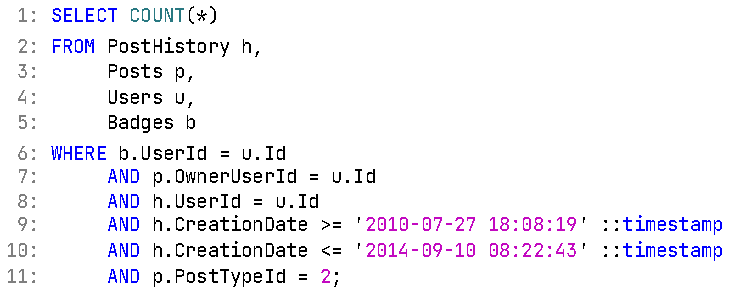
\includegraphics[scale=0.7] {fig/fig_ShowExample_Query_Full.pdf}};
    
    %%%%%%%%%%%%%%%%%%%%%%
    \node [visible on=<2->, draw=tugb, fill=tugb, line width=0.5pt, minimum width=34pt, minimum height=8pt, fill opacity=0.1] (count1) at($(sql.north west)+(61pt,-8pt)$) {};
     \node[visible on=<2->, fill=tugb!5, draw=tugb,inner sep=1mm, text=black, line width=0.5pt, right=of count1, xshift=0pt, yshift=0pt]  (pc1) {No early aggregation $\Rightarrow$ huge intermediates};
     \draw[visible on=<2->, -, tugb, line width=0.5pt, densely dashed]  (count1) -- (pc1);

    %%%%%%%%%%%%%%%%%%%%%%
    \draw[visible on=<3->, -, tug, line width=0.5pt] ($(sql.north west)+(18pt,-14pt)$) -- ($(sql.north west)+(18pt,-49pt)$) -- ($(sql.north west)+(95pt,-49pt)$) |- ($(sql.north west)+(18pt,-14pt)$);   

    \node[visible on=<3->, fill=tug!5, draw=tug,inner sep=1mm, text=black, line width=0.5pt, right=of sql, xshift=-130pt, yshift=27pt]  (p1) {Flat 4-way Cross Join};
    \draw[visible on=<3->, -, tug, line width=0.5pt, densely dashed]  ($(sql.north west)+(95pt,-25pt)$) -- (p1.west);

    %%%%%%%%%%%%%%%%%%%%%%%

    %
    \node [visible on=<4->, draw=brown, fill=brown, line width=0.5pt, minimum width=34pt, minimum height=8pt,fill opacity=0.1] (u1) at($(sql.north west)+(53pt,-36pt)$) {};
    \node [visible on=<4->, draw=brown, fill=brown, line width=0.5pt, minimum width=20pt, minimum height=8pt, fill opacity=0.1] (uid1) at($(sql.north west)+(92pt,-55pt)$) {};
    \node [visible on=<4->, draw=brown, fill=brown, line width=0.5pt, minimum width=20pt, minimum height=8pt, fill opacity=0.1] (uid2) at($(sql.north west)+(122pt,-62.5pt)$) {};
    \node [visible on=<4->, draw=brown, fill=brown, line width=0.5pt, minimum width=20pt, minimum height=8pt, fill opacity=0.1] (uid3) at($(sql.north west)+(104pt,-71pt)$) {};
   
    \node[visible on=<4->, fill=brown!5, draw=brown,inner sep=1mm, text=black, line width=0.5pt, right=of sql, xshift=-100pt, yshift=5pt]  (p2) {Join through \textbf{users} is redundant --- it is only a PK bridge};

    \draw[visible on=<4->, -, brown, line width=0.5pt, densely dashed]  (u1.east) -- (p2.west);
    \draw[visible on=<4->, -, brown, line width=0.5pt, densely dashed]  (uid1) -- (p2.west);
    \draw[visible on=<4->, -, brown, line width=0.5pt, densely dashed]  (uid2) -- (p2.west);
    \draw[visible on=<4->, -, brown, line width=0.5pt, densely dashed]  (uid3) -| (p2.west);


    %%%%%%%%%%%%%%%%%%%%%%%%%%%%%%%%%%%%%%%%%%%%%%%%%%%%%%%%%%%%%
    \node[visible on=<5->, fill=darkgreen!5, draw=darkgreen,inner sep=1mm, text=black, line width=0.5pt, right=of sql, xshift=-180pt, yshift=-75pt]  (p3) {Filters applied \textbf{after} the join};

    \node [visible on=<5->, draw=darkgreen,fill=darkgreen!30, line width=0.5pt, minimum width=198pt, minimum height=25pt, fill opacity=0.1] (filter) at($(sql.north west)+(150pt,-88pt)$) {};
    \draw[visible on=<5->, -, darkgreen, line width=0.5pt, densely dashed]  (filter) -- (p3.north);

    %%%%%%%%%%%%%%%%%%%%%%%%%%%%%%%

    \node[visible on=<6->, fill=lightgray!30,inner xsep=2mm, inner ysep=1mm, xshift=-10pt, right=of  p3, xshift=40pt, yshift=10pt]  (results) {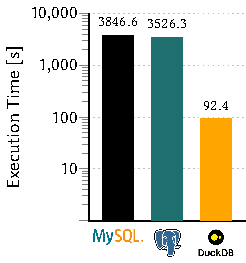
\includegraphics[scale=0.9] {fig/Experiment0-Stats122-baseline.pdf}};

  \end{tikzpicture}

%% closing line, laid over the query on the last click -- overlay, so the
%% layout above is untouched
\only<7->{%
\begin{tikzpicture}[remember picture, overlay]
  %% wash out the whole slide content, then clear a little extra right behind
  %% the band so the sentence sits on near-white
  \fill[white, opacity=0.78]
    (current page.south west) rectangle (current page.north east);
  \fill[white, path fading=softwash, opacity=0.95]
    ($(current page.center)+(-16mm,-9mm)$) ellipse (72mm and 24mm);
  \node[anchor=center, rounded corners=2.5pt, fill=tug!8, draw=tug!65,
        line width=0.7pt, inner xsep=4mm, inner ysep=2.6mm,
        font=\small\bfseries, text=tug]
    at ($(current page.center)+(-16mm,-9mm)$)
    {The optimizer is not going to save you here};
\end{tikzpicture}}
\end{frame}

%% ─── SLIDE: CHALLENGES ───────────────────────────────────────────────────────
\begin{frame}{\apptitle{black!60}{Introduction}{Challenges for Data Systems Today}}
  \footnotesize
\vspace{1mm}
\begin{columns}[T]
\begin{column}{0.45\textwidth}
  \textbf{\hblue{ML Pipeline Generation}}\\[3pt]
  \begin{itemize}\setlength\itemsep{3pt}
    \item Data prep dominates the effort
    \item LLMs hallucinate on \textbf{unseen} data
    \item AutoML searches blindly \& slowly
  \end{itemize}
\end{column}
% \hfill
\begin{column}{0.45\textwidth}
  \textbf{\hred{SQL Query Optimization}}\\[3pt]
  \begin{itemize}\setlength\itemsep{3pt}
    \item Runtime swings with query \textbf{form}
    \item Hand-written rules are brittle
    \item Rewrites must stay \textbf{equivalent}
  \end{itemize}
\end{column}
\end{columns}
\vspace{6mm}
\pause
\begin{exampleblock}{}
  \vspace{2mm}
  \centering\normalsize
  \textbf{Research vision:} make LLMs a \hgreen{reliable} component of data systems ---\\[2pt]
  \textbf{generate} like an expert, \textbf{verify} like a system.
  \vspace{2mm}
\end{exampleblock}
\end{frame}

%% ─── SLIDE: MY RESEARCH ──────────────────────────────────────────────────────
\begin{frame}{\apptitle{black!60}{Overview}{My Research --- LLM-assisted Data Systems}}
\footnotesize

\vspace{1mm}
\begin{exampleblock}{}
  \vspace{1mm}
  \centering
  \textbf{Key idea:} pair the \hgreen{creativity of LLMs} with the
  \hgreen{verification power of data systems} \\[2pt]
  generate candidates\ \faArrowRight\ verify them\ \faArrowRight\ keep only what is \textbf{correct} and \textbf{fast}.
  \vspace{1mm}
\end{exampleblock}
\vspace{4mm}

\textbf{Three systems, one recipe:}\\[4pt]

\begin{itemize}\setlength\itemsep{6pt}
  \item \hblue{CatDB}: a \textbf{data catalog} grounds the prompt; pipelines are \textbf{executed and auto-repaired} before they are accepted
  \item \hred{ReSequel}: \textbf{query templates} steer the rewrite; \textbf{sample-based checking} verifies equivalence before execution
  \item \hred{ROLEX}: rewrite \textbf{rules} are discovered from the \textbf{workload}, verified once, and then reused across queries
\end{itemize}
\end{frame}


%% ─── SLIDE 3: PREVIEW ───────────────────────────────────────────────────
\begin{frame}{\apptitle{black!60}{Overview}{Preview --- What LLM-assisted Data Systems Can Achieve}}
  \begin{tikzpicture}
    
    \node[fill=darkgreen!50,inner sep=0, line width=0.5pt,  minimum width=30pt, minimum height=32.6pt]  (automlperformance) {};
    \node[fill=darkgreen,inner sep=0, xshift=-20pt, yshift=2.8pt, line width=0.5pt, right=of automlperformance, minimum width=30pt, minimum height=39.2pt, node distance=0]  (llmperformance) {};
    \node[fill=tug,inner sep=0, xshift=-20pt, yshift=26.30pt, line width=0.5pt, right=of llmperformance, minimum width=30pt, minimum height=91.8pt, node distance=0]  (catdbperformance) {};

    \draw[{Latex[scale=1]}-, line width=1pt, black] ($(automlperformance.north west)+(-2pt,70pt)$) |- ($(catdbperformance.south east)+(2pt,0pt)$);
    % \draw[-, line width=1pt, lightgray!40] ($(automlperformance.north west)+(-2pt,80pt)$) -| ($(catdbperformance.south east)+(2pt,0pt)$); 
    
    \node[fill=none,inner sep=0, xshift=0pt, yshift=-26pt, above=of automlperformance, text=black]  {\footnotesize{32.6\%}};
    \node[fill=none,inner sep=0, xshift=0pt, yshift=-26pt, above=of llmperformance, text=black]  {\footnotesize{39.2\%}};
    \node[fill=none,inner sep=0, xshift=0pt, yshift=-26pt, above=of catdbperformance, text=black]  {\footnotesize{91.8\%}};
    \node[fill=none,inner sep=0, xshift=13pt, yshift=70pt, left=of automlperformance, text=black, rotate=90] (acc) {{\footnotesize Accuracy [\%]}};

    \node[fill=none,inner sep=0, xshift=0pt, yshift=26pt, below=of automlperformance, text=black]  {{\footnotesize AutoML}};
    \node[fill=none,inner sep=0, xshift=0pt, yshift=26pt, below=of llmperformance, text=black]  {{\footnotesize LLM}};
    \node[fill=none,inner sep=0, xshift=0pt, yshift=26pt, below=of catdbperformance, text=black]  {{\footnotesize CatDB}};

    \node[fill=none,inner sep=0, xshift=0pt, yshift=0pt, below=of llmperformance, text=black, text width=150pt]  {\footnotesize \textcolor{darkgreen}{\faCheckSquare}\ The data-centric ML pipeline generated by \textcolor{tug}{\textbf{CatDB}} improves model performance by \textcolor{blue}{52.6\%} on the Salary dataset (Example~1).};

    %%%%%%%%%%%%%%%%%%%%%%%%%%%%%%%%%%%%%%%%
    \node[visible on=<2->, fill=none,inner xsep=2mm, inner ysep=0mm, right=of  catdbperformance, xshift=20pt, yshift=0pt]  (resultsdb) {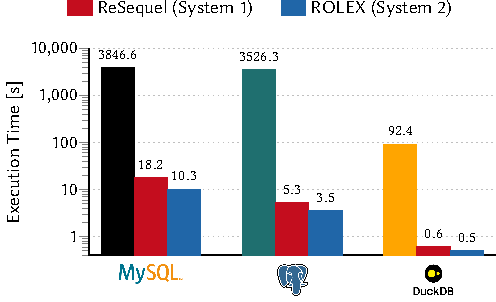
\includegraphics[scale=0.8] {fig/Experiment0-Stats122-ReSequelROLEX.pdf}};  

    \node[visible on=<2->, fill=none,inner sep=0, xshift=80pt, yshift=0pt, left=of resultsdb, text=white, rotate=90]  {\tiny MySQL Host};
    \node[visible on=<2->, fill=none,inner sep=0, xshift=134.5pt, yshift=12pt, left=of resultsdb, text=white, rotate=90]  {\tiny PostgreSQL Host};
    \node[visible on=<2->, fill=none,inner sep=0, xshift=188pt, yshift=0pt, left=of resultsdb, text=black, rotate=90]  {\tiny DuckDB Host};

    \node[visible on=<2->, fill=none,inner sep=0, xshift=0pt, yshift=10pt, below=of resultsdb, text=black, text width=220pt]  {\footnotesize
        \textcolor{darkgreen}{\faCheckSquare}\ \textcolor{tug}{\textbf{ReSequel}} rewrites the query: \textcolor{blue}{148--662$\times$} faster on DuckDB, MySQL, and PostgreSQL (Example 2).\\[6pt]
        \textcolor{darkgreen}{\faCheckSquare}\ \textcolor{tugb}{\textbf{ROLEX}} rewrites the query: \textcolor{blue}{162--998$\times$} faster.
    };
    

    
  \end{tikzpicture}
\end{frame}

%% ─── SLIDE: REST OF THIS TALK ────────────────────────────────────────────────
%% ─── THESIS CONTRIBUTIONS ────────────────────────────────────────────────────
%% Three tiles, one per contribution group.  Each tile carries the real paper
%% title, cropped straight out of the published PDF (vector, via trim/clip on
%% the extracted first page in fig/papers/), plus its venue badges.
%% \contribcard and \vbadge are defined outside the frame: beamer re-reads
%% frame bodies, where a bare #1 is illegal.
\newcommand{\vbadge}[2]{%
  \tikz[baseline=-2.5pt]\node[rounded corners=2pt, draw=#1, fill=#1!8, text=#1,
        font=\tiny\bfseries, inner xsep=3pt, inner ysep=1.6pt, line width=0.4pt]{#2};}
%% Paper screenshot with its venue stamped as a tag over the image's top-left
%% corner (the papers' own titles sit centred and lower, so nothing is hidden).
%% #1 extra white headroom (for screenshots whose title starts flush at the
%% top edge), #2 accent, #3 venue text, #4 screenshot file.
\newcommand{\ptitle}[4][0mm]{%
  \begin{tikzpicture}[baseline=(img.south)]
    \node[inner sep=0] (img) {\fboxsep=0.9mm\fcolorbox{black!12}{white}%
      {\raisebox{0pt}[\dimexpr\height+#1\relax][\depth]%
        {\includegraphics[width=\dimexpr\linewidth-2.2mm\relax]{fig/papers/#4}}}};
    \node[anchor=north west, rounded corners=1.2pt, fill=#2, text=white,
          font=\tiny\bfseries, inner xsep=2.6pt, inner ysep=1.5pt]
      at ([shift={(1.3mm,-1.3mm)}]img.north west) {#3};
  \end{tikzpicture}}
%% Bottom strip: one QR pair (paper + public code) per published system.
%% The PDFs in QRs/ are vector, so they stay crisp when the beamer is projected.
%% Each QR carries its own glyph in the centre (PDF = paper, Octocat = repo),
%% so only the system name is spelled out, centred under the pair.
%% [#1] width (13mm on the contributions strip, larger on covers), #2 accent,
%% #3 QR file.
\newcommand{\qrcell}[3][13mm]{%
  \setlength{\fboxsep}{0.35mm}%
  \fcolorbox{#2!45}{white}{\includegraphics[width=#1]{QRs/#3}}}
%% Same pair, sized for a plain cover slide and placed by the caller inside the
%% cover's tikzpicture.  #1 accent, #2 file stem in QRs/.
\newcommand{\qrcover}[2]{%
  \qrcell[14mm]{#1}{#2-paper.pdf}\hspace{2.2mm}\qrcell[14mm]{#1}{#2-code.pdf}}
%% #1 accent, #2 system name, #3 file stem in QRs/ (expects -paper and -code).
\newcommand{\qrgroup}[3]{%
  \begin{minipage}[b]{29mm}\centering
    \qrcell{#1}{#3-paper.pdf}\hspace{0.9mm}\qrcell{#1}{#3-code.pdf}\\[-1mm]
    {\scriptsize\bfseries\textcolor{#1}{#2}}%
  \end{minipage}}

\newcommand{\contribcard}[4]{% #1 accent, #2 heading, #3 strapline, #4 body
  \begin{minipage}[t]{0.317\textwidth}
    \setlength{\fboxsep}{0pt}%
    \colorbox{#1}{\makebox[\linewidth][c]{\rule[-1.3mm]{0pt}{5.2mm}%
      \color{white}\bfseries\small #2}}\\[-0.4pt]
    \setlength{\fboxsep}{2.2mm}%
    \colorbox{#1!6}{\begin{minipage}[t][37mm][t]{\dimexpr\linewidth-4.4mm\relax}
      {\tiny\itshape\textcolor{black!62}{#3}}\\[1.2mm]#4
    \end{minipage}}%
  \end{minipage}}

\begin{frame}{\apptitle{black!60}{Overview}{Thesis Contributions}}
\vspace{0.5mm}
\centering
\contribcard{tugb}{CatDB \ \textbf{+} \ GIO}{From raw data to trained models}{%
  \ptitle{tugb}{PVLDB~'25}{CatDB.png}\\[1.6mm]
  \ptitle{tugb}{SIGMOD~'25 Demo}{CatDB-demo.jpg}\\[1.6mm]
  \ptitle{tugb}{SIGMOD~'23}{GIO.png}}
\hfill
\contribcard{tug}{ReSequel}{An LLM rewrite layer over any DBMS}{%
  \ptitle{tug}{PVLDB~'26}{ReSequel.jpg}\\[2.6mm]
  {\scriptsize
   \textcolor{tug}{\ding{110}}~Rewrite once per template\\[1.1mm]
   \textcolor{tug}{\ding{110}}~Sample-verified rewrites\\[1.1mm]
   \textcolor{tug}{\ding{110}}~\textbf{2.5--16$\times$} per workload}}
\hfill
\contribcard{darkgreen}{ROLEX}{Distilling those rewrites into rules}{%
  \ptitle[3.4mm]{darkgreen}{SIGMOD~'27 --- under submission}{Rolex.png}\\[2.6mm]
  {\scriptsize
   \textcolor{darkgreen}{\ding{110}}~Offline LLM $\to$ C++ rules\\[1.1mm]
   \textcolor{darkgreen}{\ding{110}}~Zero LLM cost at runtime\\[1.1mm]
   \textcolor{darkgreen}{\ding{110}}~\textbf{60\%} below ReSequel}}

\vspace{1.2mm}
\makebox[\textwidth]{%
  \qrgroup{tugb}{CatDB}{CatDB}\hspace{5mm}%\hfill
  \qrgroup{tugb}{GIO}{GIO}\hspace{5mm}
  \qrgroup{tug}{ReSequel}{ReSequel}}

% \vspace{0.6mm}
% \begin{exampleblock}{}
%   \centering\footnotesize
%   One recipe across all four systems: \hgreen{generate like an expert}, \hgreen{verify like a system}
% \end{exampleblock}
\end{frame}

%%%%%%%%%%%%%%%%%%%%%%%%%%%%%%%%%%%%%%%%%%%%%%%%%%%%%%%%%%%%%%%%%%%%%%%%%%%
%% ════ PART 1: CatDB ════
%%%%%%%%%%%%%%%%%%%%%%%%%%%%%%%%%%%%%%%%%%%%%%%%%%%%%%%%%%%%%%%%%%%%%%%%%%%
%% Paper cover slide.  The decorative circles are laid out relative to the page
%% corners, so the same block can be reused for ReSequel/ROLEX by swapping the
%% accent color, the title, and the venue/author block.
\begin{frame}[plain,noframenumbering]
\begin{tikzpicture}[remember picture, overlay]
  %% ── background: big corner disc + three accent circles ──
  \begin{scope}
    \clip (current page.south west) rectangle (current page.north east);
    \fill[black!58] ($(current page.north east)+(-22mm, 8mm)$) circle (48mm);
    \fill[tugb]     ($(current page.north west)+( 24mm,-22mm)$) circle (13mm);
    \fill[color4]   ($(current page.north west)+( 51mm,-39mm)$) circle (8mm);
    \fill[gray!60]  ($(current page.north west)+( 69mm,-32mm)$) circle (2.5mm);
  \end{scope}

  %% ── full publication title, right-aligned against the rule ──
  \node[anchor=south east, text width=94mm, align=right, inner sep=0, text=black]
    at ($(current page.south west)+(97mm,11mm)$)
    {\large\bfseries \textcolor{tugb}{CatDB:} Data-catalog-guided, LLM-based Generation of Data-centric ML Pipelines};

  %% ── separator ──
  \draw[black, line width=0.6pt]
    ($(current page.south west)+(101mm,10mm)$) -- ++(0mm,29mm);

  %% ── venue + authors ──
  \node[anchor=north west, text width=48mm, align=left, inner sep=0, text=black]
    at ($(current page.south west)+(106mm,39mm)$)
    {{\normalsize\itshape \textcolor{tugb}{PVLDB '25}}\\[2pt]
     {\normalsize\itshape \textcolor{tugb}{SIGMOD '25 (Demo)}}\\[8pt]
     {\small\textbf{Saeed Fathollahzadeh}\\[2pt]
      \small Essam Mansour\\[2pt]
      \small Matthias Boehm}};

  % ── paper + code QR pair (left, clear of the title block) ──
  \node[anchor=south west, inner sep=0]
    at ($(current page.south west)+(65mm,25mm)$) {\qrcover{tugb}{CatDB}};
\end{tikzpicture}
\end{frame}


\begin{frame}{\apptitle{tugb}{CatDB}{Motivation}}
 \tiny
 \centering
 \resizebox{\linewidth}{!}{
  \begin{tikzpicture}
    \node[fill=white,inner sep=0, text=black, xshift=-10pt, line width=0.5pt]  (ds) {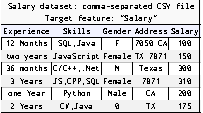
\includegraphics[scale=1.2] {fig/fig_salary_ds.pdf}};

    \node[draw=lightgray,fill=tugb!10,inner sep=1mm, text=black, right=of ds, xshift=2pt]  (description) {
      \shortstack[l]{\textbf{Generate a data science pipeline.}\\[3pt]
      \textcolor{black}{Experience} $\to$ \textcolor{tug}{string}, \texttt{100\%} distinct\\
      \textcolor{black}{Skills}$\to$ \textcolor{tug}{string}, \texttt{100\%} distinct\\
      \textcolor{black}{Gender}$\to$ \textcolor{tug}{categorical}, \texttt{60\%} distinct\\
      \textcolor{black}{Address}$\to$ \textcolor{tug}{string}, \texttt{100\%} distinct\\[3pt]
      \textbf{Build an ensemble model to forecast \textcolor{blue}{salary}.}
      }
      };
    
    \draw[-{Latex[scale=.6]}, line width=0.65pt, tugb] ($(description.north west)+(-32pt,-6pt)$) -- ($(description.north west)+(3pt,-6pt)$);  

    \draw[-{Latex[scale=.6]}, line width=0.65pt, tugb] ($(description.south west)+(-32pt,6pt)$) -- ($(description.south west)+(3pt,6pt)$);  

    \draw[{Latex[scale=.6]}-{Latex[scale=.6]}, line width=0.65pt, tugb] ($(description.north west)+(3pt,-18pt)$) -- ($(description.north west)+(-3pt,-18pt)$) -- ($(description.south west)+(-3pt,18pt)$) -- ($(description.south west)+(3pt,18pt)$); 

    \draw[-, line width=0.65pt, tugb] ($(description.west)+(-32pt,0pt)$) -- ($(description.west)+(-3pt,0pt)$);  

    \node[fill=none,inner sep=0, text=tugb] at ($(description.north west)+(-20pt,0pt)$)  (task) {Task};
    \node[fill=none,inner sep=0, text=tugb] at ($(description.south west)+(-15pt,0pt)$)  (prompt) {Prompt};
    \node[fill=none,inner sep=0, text=tugb] at ($(description.west)+(-18pt,4pt)$)  (metadata) {Metadata};

    %%%%%%%%%%%%%%%%%%%%%%%%%%%%
    \node[fill=white,inner sep=0,xshift=-10pt, right=of description ]  (llm) {
\includegraphics[scale=1.2] {fig/fig_LLM.pdf}};
    \draw[-{Latex[scale=.7]}, line width=0.8pt, tugb] (description) -- (llm);

    \node[draw=lightgray,fill=lightgray!40,inner sep=1.5mm,xshift=-10pt, right=of llm ]  (pipeline) {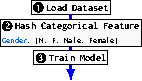
\includegraphics[scale=1.2] {fig/fig_metadata_pipDAG.pdf}};
    \draw[-{Latex[scale=.7]}, line width=0.8pt, tugb] (llm) -- (pipeline);  
    
    %%%%%%%%%%%%%%%%%%%%%%%%%%%%%%%%%%%%

     \node[visible on=<2->, rectangle callout, rounded corners=2pt,
           callout absolute pointer={($(llm.north)+(0pt,2pt)$)},
           callout pointer width=8pt,
           fill=brown!7, draw=brown, line width=0.5pt, text=black, inner sep=1.5mm,
           anchor=south, text width=107pt] at ($(llm.north)+(0pt,34pt)$)  (b1) {\textbf{Never seen before} --- LLMs memorized public benchmarks (Titanic), not \textit{your} private dataset};

        \node[visible on=<3->, rectangle callout, rounded corners=2pt,
           callout absolute pointer={($(description.west)+(10pt,0pt)$)},
           callout pointer width=8pt,
           fill=brown!7, draw=brown, line width=0.5pt, text=black, inner sep=1.5mm,
           anchor=south, text width=107pt] at ($(description.north)+(-35pt,10pt)$)  (b2) {\textbf{Noisy, incomplete metadata} --- basic types, hide semantics (categorical, list); dirty distinct value};    
      
      \node[visible on=<4->, fill=tug, draw=tug,inner sep=0, fill opacity=0.05, minimum width=29pt, minimum height=50pt, line width=0.7pt] at ($(ds.north west)+(15pt,-40pt)$) (experience) {}; 

      \node[visible on=<4->, fill=tug, draw=tug,inner sep=0, fill opacity=0.05, minimum width=18pt, minimum height=50pt, line width=0.7pt] at ($(ds.north west)+(68.5pt,-40pt)$) (gender) {};

      \node[visible on=<4->, rectangle callout, rounded corners=2pt,
           callout absolute pointer={($(experience.south)+(0pt,0pt)$)},
           callout pointer width=8pt,
           fill=tug!7, draw=tug, line width=0.5pt, text=black, inner sep=1.5mm,
           anchor=north, text width=90pt, align=left] at ($(experience.south)+(35pt,-24pt)$)  (expb1) {\textbf{Semantically equivalent values}\\[2pt]
           \texttt{36 months} $\equiv$ \texttt{3 Years}, \\ \texttt{F} $\equiv$ \texttt{Female}, \\ ... \\[2pt]
           100\% distinct hides categorical};

      %% second callout tail: same balloon also points to the Gender column
      \coordinate (gtip)  at ($(gender.south)+(0pt,-1pt)$);
      \coordinate (gbase) at (expb1.north -| gender.south);
      \fill[visible on=<4->, tug!7] ($(gbase)+(-4pt,0.5pt)$) -- (gtip) -- ($(gbase)+(4pt,0.5pt)$) -- cycle;
      \draw[visible on=<4->, tug!7, line width=1pt] ($(gbase)+(-4pt,0pt)$) -- ($(gbase)+(4pt,0pt)$);
      \draw[visible on=<4->, tug, line width=0.5pt] ($(gbase)+(-4pt,0pt)$) -- (gtip) -- ($(gbase)+(4pt,0pt)$);
      %%%%%%%%%%%%%%%%%%%%%%%%%%%%%%%%%%%%%%%%%%%%%%%%%%%%%%%%%%%%
      
      \node[visible on=<5->, fill=tugb, draw=tugb,inner sep=0, fill opacity=0.05, minimum width=28pt, minimum height=50pt, line width=0.7pt] at ($(ds.north west)+(44.5pt,-40pt)$) (skills) {}; 
      
      \node[visible on=<5->, rectangle callout, rounded corners=2pt,
           callout absolute pointer={($(skills.north)+(10pt,0pt)$)},
           callout pointer width=8pt,
           fill=tugb!7, draw=tugb, line width=0.5pt, text=black, inner sep=1.5mm,
           anchor=south, text width=78pt, align=left] at ($(skills.north)+(0pt,20pt)$)  (skb1) {\textbf{Sentence, not a plain string}\\[2pt]
           \texttt{SQL,Java} $\to$ \textbf{list} feature};

      \node[visible on=<6->, fill=darkgreen, draw=darkgreen,inner sep=0, fill opacity=0.05, minimum width=20pt, minimum height=50pt, line width=0.7pt] at ($(ds.north west)+(88pt,-40pt)$) (address) {};

       \node[visible on=<6->, rectangle callout, rounded corners=2pt,
           callout absolute pointer={($(address.south)+(0pt,0pt)$)},
           callout pointer width=8pt,
           fill=darkgreen!7, draw=darkgreen, line width=0.5pt, text=black, inner sep=1.5mm,
           anchor=north, text width=85pt, align=left] at ($(address.south)+(65pt,-36pt)$)  (adb1) {\textbf{Composite, not a plain string}\\[2pt]
           \texttt{7050 CA} $\to$ \texttt{Zip} + \texttt{State}};
    %%%%%%%%%%%%%%%%%%%%%%%%%%%%%%%%%%%%%%%%%
         \node[visible on=<7->, rectangle callout, rounded corners=2pt,
           callout absolute pointer={($(description.south)+(-20pt,4pt)$)},
           callout pointer width=8pt,
           fill=brown!7, draw=brown, line width=0.5pt, text=black, inner sep=1.5mm,
           anchor=south, text width=125pt] at ($(description.south)+(30pt,-30pt)$)  (b3) {\textbf{Generic prompts $\to$ generic pipelines} \\[2pt] need per-stage, dataset-specific instructions};       
  \end{tikzpicture}
 }

\vspace{1mm}
\begin{exampleblock}{}<8->
  \centering\large
  \textbf{Data catalogs} store profiling info that can \hgreen{precisely guide} LLMs
\end{exampleblock}
\end{frame}

%%%%%%%%%%%%%%%%%%%%%%%%%%%%%%%%%%%%%%%%%%%%%%%%%%%%%%%%%%%
\begin{frame}{\apptitle{tugb}{CatDB}{LLM-based Generation of Data-centric ML Pipelines}}

  \begin{itemize}
    \item {\footnotesize \textbf{Zero-shot in-context learning} --- no task-specific examples, no fine-tuning:  the \textcolor{tugb}{data catalog} guides the LLM, and \textcolor{tugb}{execution} verifies it.}
  \end{itemize}  

\vspace{3mm}
    \tiny
    \centering
    \resizebox{\linewidth}{!}{
    \begin{tikzpicture}

        %% Drawn back-to-front: stage 3 first, stage 1 last, so each arrow band
        %% is overlapped by the *earlier* stage rather than the later one.
        %% Reveal order is independent of draw order (visible on=<n->).

        %% ── stage 3: Manage Pipeline (bottom of the stack, revealed last) ──
        \draw[visible on=<3->, -{Triangle[width=2*8.1pt,length=10pt]}, line width=17pt, tug] (10.95,0) -- (14.5,0);
        \node[visible on=<3->, fill=none,inner sep=0] at(12.6,-2.6) (arch3) {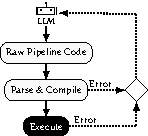
\includegraphics[scale=1.2]{figures/img/fig_PipelineDAG.pdf}};
        \draw[visible on=<3->, -, line width=1pt, tug] (11,-0.28) -- (11,-4.8) -- (14.15,-4.8) -- (14.15,-0.20);

        %% ── stage 2: Prompt Construction ──
        \draw[visible on=<2->, -{Triangle[width=2*8.1pt,length=10pt]}, line width=17pt, tug!40] (1.9,0) -- (11.3,0);
        \node[visible on=<2->, fill=none,inner sep=0] at(7,-2.6) (arch2) {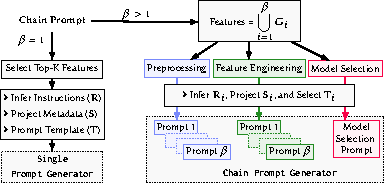
\includegraphics[scale=1.2]{figures/img/fig_PromptDAG.pdf}};
        \draw[visible on=<2->, -, line width=1pt, tug!40] (2.7,-0.28) -- (2.7,-4.8) -- (10.95,-4.8) -- (10.95,-0.20);

        %% ── stage 1: Data Catalog (top of the stack, shown from the start) ──
        \draw[-{Triangle[width=2*8.1pt,length=10pt]}, line width=17pt, tug!20] (0,0) -- (3,0);
        \node[fill=none,inner sep=0] at(1.3,-2.6) (arch1) {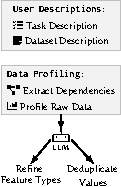
\includegraphics[scale=1.2]{figures/img/fig_DataCatalog.pdf}};
        \draw[-, line width=1pt, tug!20] (0.02,-0.28) -- (0.02,-4.8) -- (2.63,-4.8) -- (2.63,-0.20);

        %% ── stage labels last, so they sit on top of every band ──
        \node[fill=none,inner sep=0] at(1.3,0) {\footnotesize{\textbf{Data Catalog}}};
        \node[visible on=<2->, fill=none,inner sep=0] at(7,0) {\footnotesize{\textbf{Prompt Construction}}};
        \node[visible on=<3->, fill=none,inner sep=0, text=white] at(12.8,0) {\footnotesize{\textbf{Manage Pipeline}}};
        
    \end{tikzpicture}
    }

\end{frame}

\begin{frame}{\apptitle{tugb}{CatDB}{Schema Refinement}}
\vspace{0mm}

%% ── refinement example, pinned to the top-right corner of the page ──
\begin{tikzpicture}[remember picture, overlay]
  \node[anchor=north east, inner sep=0]
        at ($(current page.north east)+(-5mm,-10mm)$)
        {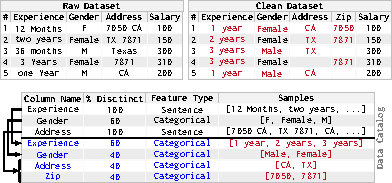
\includegraphics[width=0.50\paperwidth]{fig/fig_cleaning_example.pdf}};
\end{tikzpicture}

\vspace{-7mm}
%% ── left: problem and approach ───────────────────────────────────────
\begin{minipage}[t]{1\textwidth}
  % \scriptsize
  \footnotesize
  \begin{itemize}
  \item \textbf{Problems}\\[2pt]
  \begin{itemize}\setlength\itemsep{2pt}
    \item {\footnotesize \textcolor{tug}{\textbf{\#1 Different representations}} \\[1pt] \textcolor{gray!150}{ for the same categorical value}} \\[4pt]
    \item {\footnotesize \textcolor{tug}{\textbf{\#2 Concatenated lists}} / \\[1pt] \textcolor{gray!150}{composite features}}
  \end{itemize}

  \pause
  \vspace{3mm}
  \item \textbf{Approach}\\[2pt]
  \begin{itemize}\setlength\itemsep{2pt}
    \item {\footnotesize Identify candidate \textbf{string} features}
    \item {\footnotesize Build a prompt from the feature name and its distinct values}
    \item {\footnotesize \textcolor{tug}{Let the LLM} (GPT, Gemini, Llama) \textcolor{tug}{create a mapping} from the original to a reduced value set, and infers the \textcolor{tugb}{feature type} \faArrowRight \textcolor{tug}{\textbf{\ Iterative refinement}}}
  \end{itemize}
\end{itemize}
\end{minipage}

\vspace{3mm}
%% Catalog refinement: distinct values per column, EU IT dataset only
{\centering
\resizebox{0.9\linewidth}{!}{%
\addtolength{\tabcolsep}{0.5em}
  \begin{tabular}{c|cccccccccccccc}
    \toprule
    \textbf{Method} & \#1 & \#2 & \#3 & \#4 & \#5 & \#6 & \#7 & \#8 & \#9 & \#10 & \#11 & \#12 & \#13 & \#14 \\ \midrule
    Original & \cellcolor{tugb!20}563 & 256 & 148 & 64 & 119 & 53 & 59 & 46 & 24 & 11 & 48 & 12 & 15 & 4 \\
    \textbf{CatDB} & \cellcolor{tugb!20}\textbf{100} & 43 & 45 & 32 & 95 & 39 & 47 & 36 & 16 & 3 & 43 & 6 & 9 & 3 \\
    \bottomrule
  \end{tabular}%
}
\par}
\end{frame}


\begin{frame}{\apptitle{tugb}{CatDB}{Prompt Construction and Pipeline Management}}
% \vspace{-2mm}

{\scriptsize
\begin{itemize}
  \item \textbf{Rules (R)} + \textbf{schema (S)} in template \textbf{T}: coding task per stage $+$ refined catalog\\[3pt]

  \item \textbf{Validate}: syntax check, then \textbf{execute} on the local dataset\\[3pt]

  \item \textbf{Repair loop}: knowledge-base patches; syntax/runtime
          errors re-prompted with the catalog slice
\end{itemize}  
}
\vspace{2mm}
\centering
\begin{tikzpicture}[node distance=3mm]
      %% prompt example: exactly half the slide width
      \node[inner sep=0pt] (prompt) {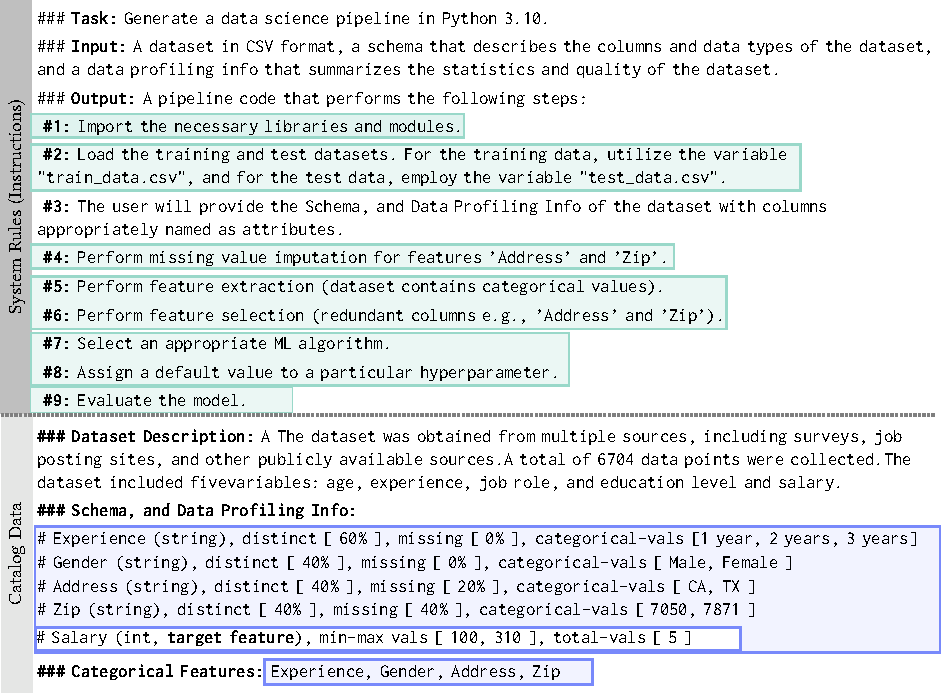
\includegraphics[width=0.5\linewidth]{fig/fig_prompt_example.pdf}};
      %% pipeline DAG: width chosen so its height matches the prompt figure
      \node[fill=tugb!7,inner sep=2pt, right=of prompt, xshift=40pt] (dag) {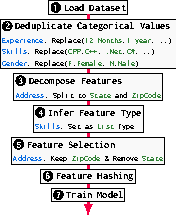
\includegraphics[width=0.29\linewidth]{fig/fig_catdb_pipDAG.pdf}};

      %% rotated label glued to the right edge of (dag), centred on its height
      \node[text=gray, inner sep=0, rotate=90, anchor=north] at ($(dag.east)+(2pt,0pt)$)
            {{\scriptsize \textbf{Pipeline DAG with CatDB and LLM}}};
      
      %% fat arrow: prompt feeds the LLM, which yields the pipeline DAG
      \draw[-{Triangle[width=2*9pt,length=11pt]}, line width=11pt, tug]
            ($(prompt.east)+(4pt,0pt)$) -- ($(dag.west)-(6pt,0pt)$);
\end{tikzpicture}

% \vspace{1mm}
\begin{exampleblock}{}
  \centering\scriptsize
  CatDB-generated prompt (instructions $+$ refined metadata) for the \textbf{Salary}
  dataset, and the resulting pipeline
\end{exampleblock}

%% ── final overlay: dim the slide and show the accuracy result on top ──
\only<2>{%
\begin{tikzpicture}[remember picture, overlay]

  %% frosted-glass wash over everything already on the slide
  \fill[white, opacity=0.85]
        (current page.south west) rectangle (current page.north east);

  %% the result plot, floating above the dimmed slide
  \node[fill=white, draw=tug, line width=0.8pt, rounded corners=4pt,
        inner sep=7mm, drop shadow={opacity=0.25, shadow xshift=1.5pt, shadow yshift=-1.5pt}]
       at (current page.center) {%
    %% sharp corners: the frame's rounding must not leak into the bars/axis
    \begin{tikzpicture}[sharp corners]

    \node[fill=darkgreen!50,inner sep=0, line width=0.5pt,  minimum width=30pt, minimum height=32.6pt]  (automlperformance) {};
    \node[fill=darkgreen,inner sep=0, xshift=-20pt, yshift=2.8pt, line width=0.5pt, right=of automlperformance, minimum width=30pt, minimum height=39.2pt, node distance=0]  (llmperformance) {};
    \node[fill=tug,inner sep=0, xshift=-20pt, yshift=26.30pt, line width=0.5pt, right=of llmperformance, minimum width=30pt, minimum height=91.8pt, node distance=0]  (catdbperformance) {};

    \draw[{Latex[scale=1]}-, line width=1pt, black] ($(automlperformance.north west)+(-2pt,70pt)$) |- ($(catdbperformance.south east)+(2pt,0pt)$);

    \node[fill=none,inner sep=0, xshift=0pt, yshift=-26pt, above=of automlperformance, text=black]  {\footnotesize{32.6\%}};
    \node[fill=none,inner sep=0, xshift=0pt, yshift=-26pt, above=of llmperformance, text=black]  {\footnotesize{39.2\%}};
    \node[fill=none,inner sep=0, xshift=0pt, yshift=-26pt, above=of catdbperformance, text=black]  {\footnotesize{91.8\%}};
    \node[fill=none,inner sep=0, xshift=13pt, yshift=70pt, left=of automlperformance, text=black, rotate=90] (acc) {{\footnotesize Accuracy [\%]}};

    \node[fill=none,inner sep=0, xshift=0pt, yshift=26pt, below=of automlperformance, text=black]  {{\footnotesize AutoML}};
    \node[fill=none,inner sep=0, xshift=0pt, yshift=26pt, below=of llmperformance, text=black]  {{\footnotesize LLM}};
    \node[fill=none,inner sep=0, xshift=0pt, yshift=26pt, below=of catdbperformance, text=black]  {{\footnotesize CatDB}};

    \end{tikzpicture}%
  };
\end{tikzpicture}}
\end{frame}

%%%%%%%%%%%%%%%%%%%%%%%%%%%%
\begin{frame}{\apptitle{tugb}{CatDB}{Performance Comparison (LLM = Gemini-1.5)}}
    \centering
    
\includegraphics[width=0.99\linewidth]{plots/Experiment-Slide-Clean-Legend}\\[3pt]

    \begin{minipage}[t]{0.33\linewidth}\centering
      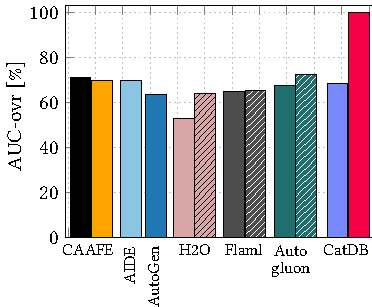
\includegraphics[width=\linewidth]{plots/Experiment-Slide-Etailing}\\[1pt]
      {\scriptsize \textbf{Etailing}}
    \end{minipage}\hfill
    \begin{minipage}[t]{0.33\linewidth}\centering
      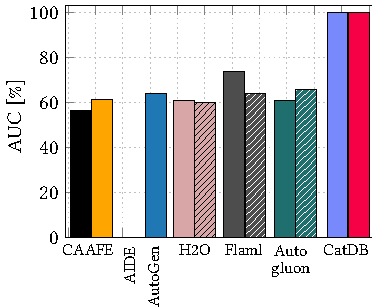
\includegraphics[width=\linewidth]{plots/Experiment-Slide-WiFi}\\[1pt]
      {\scriptsize \textbf{Wifi}}
    \end{minipage}\hfill
    \begin{minipage}[t]{0.33\linewidth}\centering
      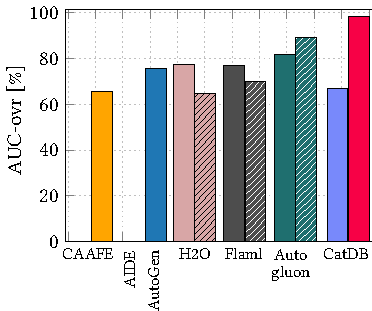
\includegraphics[width=\linewidth]{plots/Experiment-Slide-Yelp}\\[1pt]
      {\scriptsize \textbf{Yelp}}
    \end{minipage}

    \vspace{2mm}
    \raggedright\scriptsize

    \begin{itemize}
      \item  \textcolor{blue}{\textbf{Deduplication} \ding{220}} Removes duplicates, balances labels.
      \item \textcolor{blue}{\textbf{Categorical Features} \ding{220}} Fixes formatting, transforms complexity.
      \item \textcolor{blue}{\textbf{Feature Refinement} \ding{220}} Drops constant/misread features, preserves distribution. 
    \end{itemize}  
\end{frame}

% %%%%%%%%%%%%%%%%%%%%%%%%%%%%%%%%%%%%%%%%%%%%%%%%%%%%%%%%%%%%%%%%%%%%%%
\begin{frame}{\apptitle{tugb}{CatDB}{Outlier and Missing Value Injection (Gemini-1.5)}}
\centering

\includegraphics[width=0.99\linewidth]{plots/Experiment5-Legend}\\[4pt]

\begin{minipage}[t]{0.44\linewidth}\centering
  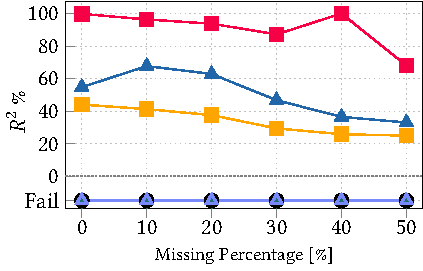
\includegraphics[width=\linewidth]{plots/Experiment-Slide-Utility-MVOUT.pdf}\\[1pt]
  {\scriptsize (a) \textbf{Utility MV $+$ Outlier $=5\%$}} \hfill
\end{minipage}\hspace{0.06\linewidth}
\begin{minipage}[t]{0.44\linewidth}\centering
  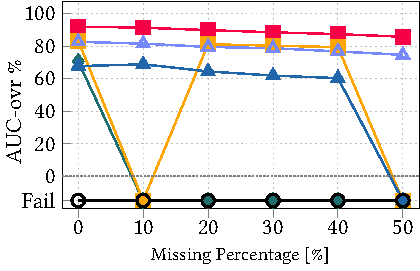
\includegraphics[width=\linewidth]{plots/Experiment-Slide-Volkert-MVOUT.pdf}\\[1pt]
  {\scriptsize (b) \textbf{Volkert MV $+$ Outlier $=5\%$}}
\end{minipage}

\vspace{7mm}
\raggedright\scriptsize
\ding{110} \textcolor{blue}{\textbf{Robustness} \ding{220}} CatDB maintains high performance
even with increasing missing values and 5\% outliers.
\end{frame}


%%%%%%%%%%%%%%%%%%%%%%%%%%%%%%%%%%%%%%%%%%%%%%%%%%%%%%%%%%%%%%%%%%%%%%%%%%%
%% ════ PART 2: ReSequel ════
%%%%%%%%%%%%%%%%%%%%%%%%%%%%%%%%%%%%%%%%%%%%%%%%%%%%%%%%%%%%%%%%%%%%%%%%%%%
\begin{frame}[plain,noframenumbering]
\begin{tikzpicture}[remember picture, overlay]
  %% ── background: big corner disc + three accent circles ──
  \begin{scope}
    \clip (current page.south west) rectangle (current page.north east);
    \fill[black!58] ($(current page.north east)+(-22mm, 8mm)$) circle (48mm);
    \fill[tugb]     ($(current page.north west)+( 24mm,-22mm)$) circle (13mm);
    \fill[color4]   ($(current page.north west)+( 51mm,-39mm)$) circle (8mm);
    \fill[gray!60]  ($(current page.north west)+( 69mm,-32mm)$) circle (2.5mm);
  \end{scope}

  %% ── full publication title, right-aligned against the rule ──
  \node[anchor=south east, text width=94mm, align=right, inner sep=0, text=black]
    at ($(current page.south west)+(97mm,11mm)$)
    {\large\bfseries \textcolor{tug}{ReSequel:} Robust LLM-assisted Query Rewriting and Optimization using Templatization and Sampling};

  %% ── separator ──
  \draw[black, line width=0.6pt]
    ($(current page.south west)+(101mm,10mm)$) -- ++(0mm,29mm);

  %% ── venue + authors ──
  \node[anchor=north west, text width=48mm, align=left, inner sep=0, text=black]
    at ($(current page.south west)+(106mm,39mm)$)
    {{\normalsize\itshape \textcolor{tugb}{PVLDB '26}}\\[8pt]
     {\small\textbf{Saeed Fathollahzadeh}\\[2pt]
      \small Essam Mansour\\[2pt]
      \small Matthias Boehm}};

  %% ── paper + code QR pair (left, clear of the title block) ──
  \node[anchor=south west, inner sep=0]
    at ($(current page.south west)+(65mm,29mm)$) {\qrcover{tug}{ReSequel}};
\end{tikzpicture}
\end{frame}

%% ─── MOTIVATION FOR ReSequel ─────────────────────────────────────────────────
%% Survey of the 21 "messy query rewrite objectives" (6 categories) from the
%% ReSequel paper: how much of each category today's rewriters actually cover.
%% Scoring: full support = 1, partial (+/-) = 0.5, none = 0.
\begin{frame}{\apptitle{tug}{ReSequel}{Motivation --- What Do Query Rewriters Actually Cover?}}
\vspace{2mm}
\centering
%% scale the whole picture to 95\% of the frame's usable height
\resizebox{!}{0.80\textheight}{%
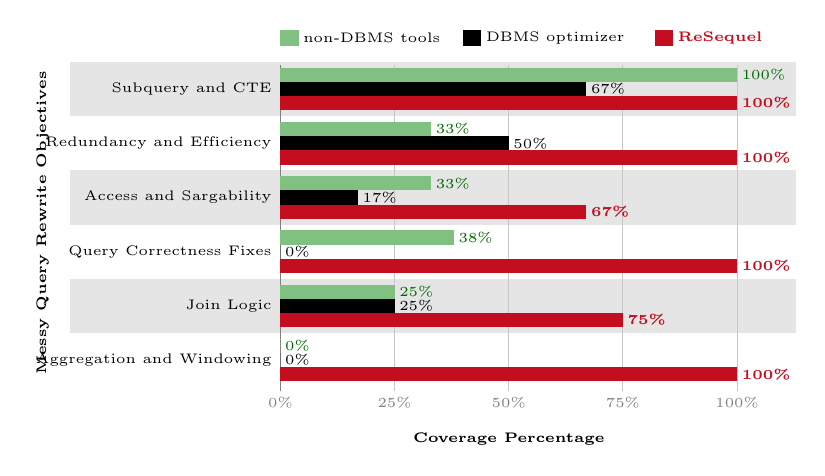
\begin{tikzpicture}[x=0.58mm, y=0.82mm, font=\scriptsize]

  \def\barh{2.2}
  \def\gp{0}      % no gap: the three bars of a category touch
  \def\pitch{8.4}

  %% ── alternating band behind every other category, for readability ──
  \foreach \i in {0,...,5} {
    \pgfmathtruncatemacro{\isodd}{mod(\i,2)}
    \ifnum\isodd=0
      \pgfmathsetmacro{\bandb}{(5-\i)*\pitch+3-0.9}
      \pgfmathsetmacro{\bandt}{\bandb+3*\barh+1.8}
      \fill[lightgray!40] (-46,\bandb) rectangle (113,\bandt);
    \fi
  }

  %% ── legend ──
  \fill[darkgreen!50] (0,55) rectangle (4,57.4);
  \node[right, font=\tiny, inner sep=1.5pt] at (4,56.2) {non-DBMS tools};
  \fill[black]  (40,55) rectangle (44,57.4);
  \node[right, font=\tiny, inner sep=1.5pt] at (44,56.2) {DBMS optimizer};
  \fill[visible on=<2->, tug] (82,55) rectangle (86,57.4);
  \node[visible on=<2->, right, font=\tiny, inner sep=1.5pt, text=tug] at (86,56.2) {\textbf{ReSequel}};

  %% ── grid + axis ──
  \foreach \v in {0,25,50,75,100} {
    \draw[lightgray!90, line width=0.4pt] (\v,1.5) -- (\v,52);
    \node[below, font=\tiny, text=gray, inner sep=2pt] at (\v,1.5) {\v\%};
  }
  \draw[gray, line width=0.4pt] (0,1.5) -- (0,52);

  %% ── axis labels ──
  \node[below, font=\tiny, inner sep=1pt] at (50,-4.5)
       {\textbf{Coverage Percentage}};
  \node[rotate=90, anchor=south, font=\tiny, inner sep=1pt] at (-50,27.5)
       {\textbf{Messy Query Rewrite Objectives}};

  %% ── one group of three bars per category ──
  %% listed top-to-bottom: first entry is the topmost category
  \foreach [count=\i from 0] \cat/\a/\b/\c in {%
      {Subquery and CTE}/100/67/100,
      {Redundancy and Efficiency}/33/50/100,
      {Access and Sargability}/33/17/67,
      {Query Correctness Fixes}/38/0/100,
      {Join Logic}/25/25/75,
      {Aggregation and Windowing}/0/0/100}
  {
    \pgfmathsetmacro{\yc}{(5-\i)*\pitch+3}
    \pgfmathsetmacro{\yb}{\yc+\barh+\gp}
    \pgfmathsetmacro{\ya}{\yc+2*\barh+2*\gp}
    \pgfmathsetmacro{\yat}{\ya+\barh}
    \pgfmathsetmacro{\ybt}{\yb+\barh}
    \pgfmathsetmacro{\yct}{\yc+\barh}
    \pgfmathsetmacro{\yam}{\ya+0.5*\barh}
    \pgfmathsetmacro{\ybm}{\yb+0.5*\barh}
    \pgfmathsetmacro{\ycm}{\yc+0.5*\barh}
    \pgfmathsetmacro{\ylab}{\yb+0.5*\barh}

    \fill[darkgreen!50] (0,\ya) rectangle (\a,\yat);
    \fill[black]  (0,\yb) rectangle (\b,\ybt);
    \fill[visible on=<2->, tug] (0,\yc) rectangle (\c,\yct);

    \node[right, font=\tiny, text=darkgreen!80!black, inner sep=1.5pt] at (\a,\yam) {\a\%};
    \node[right, font=\tiny, text=black,           inner sep=1.5pt] at (\b,\ybm) {\b\%};
    \node[visible on=<2->, right, font=\tiny, text=tug, inner sep=1.5pt] at (\c,\ycm) {\textbf{\c\%}};

    \node[left, font=\tiny, inner sep=3pt] at (0,\ylab) {\cat};
  }

  % \pause

\end{tikzpicture}}

%% ── final overlay: dim the per-category chart and show the overall coverage ──
\only<3>{%
\begin{tikzpicture}[remember picture, overlay]

  %% frosted-glass wash over the chart behind
  \fill[white, opacity=0.86]
        (current page.south west) rectangle (current page.north east);

  \node[fill=white, draw=tug, line width=0.8pt, rounded corners=4pt, inner sep=6mm,
        drop shadow={opacity=0.25, shadow xshift=1.5pt, shadow yshift=-1.5pt}]
       at (current page.center) {%
    %% sharp corners: the frame's rounding must not leak into the bars
    \begin{tikzpicture}[sharp corners]

      \node[inner sep=0, anchor=south, font=\small] at (44pt,104pt)
           {\textbf{Overall coverage of the \numprint{21} rewrite objectives}};

      %% axis
      \draw[{Latex[scale=0.8]}-, line width=0.7pt, black]
           (-14pt,96pt) |- (104pt,0pt);
      \node[rotate=90, anchor=south, font=\scriptsize, inner sep=2pt] at (-16pt,44pt)
           {Coverage [\%]};

      %% bars: value x 0.8pt
      \node[fill=darkgreen!50, inner sep=0, anchor=south,
            minimum width=26pt, minimum height=30.4pt] at (10pt,0pt)  (a) {};
      \node[fill=black,        inner sep=0, anchor=south,
            minimum width=26pt, minimum height=19.2pt] at (46pt,0pt)  (b) {};
      \node[fill=tug,          inner sep=0, anchor=south,
            minimum width=26pt, minimum height=70.4pt] at (82pt,0pt)  (c) {};

      %% values on top
      \node[above, font=\scriptsize, inner sep=2pt, text=darkgreen!60!black] at (a.north) {\textbf{38\%}};
      \node[above, font=\scriptsize, inner sep=2pt, text=black]              at (b.north) {\textbf{24\%}};
      \node[above, font=\scriptsize, inner sep=2pt, text=tug]                at (c.north) {\textbf{88\%}};

      %% names below
      \node[below, font=\scriptsize, inner sep=3pt] at (a.south) {non-DBMS};
      \node[below, font=\scriptsize, inner sep=3pt] at (b.south) {DBMS};
      \node[below, font=\scriptsize, inner sep=3pt, text=tug] at (c.south) {\textbf{ReSequel}};

      % \node[below, font=\tiny, inner sep=1pt, text=gray] at (44pt,-12pt)
      %      {full $=1$, partial $=0.5$, none $=0$};
    \end{tikzpicture}%
  };
\end{tikzpicture}}
\end{frame}

%% ─── SLIDE 13: ReSequel SOLUTION ─────────────────────────────────────────────
\begin{frame}{\vspace{-2mm} \apptitle{tug}{ReSequel}{LLM Rewriting as an Outer Optimization Layer}}
  \vspace{-2mm}

  \begin{tikzpicture}
    \node[visible on=<5>] (orig) {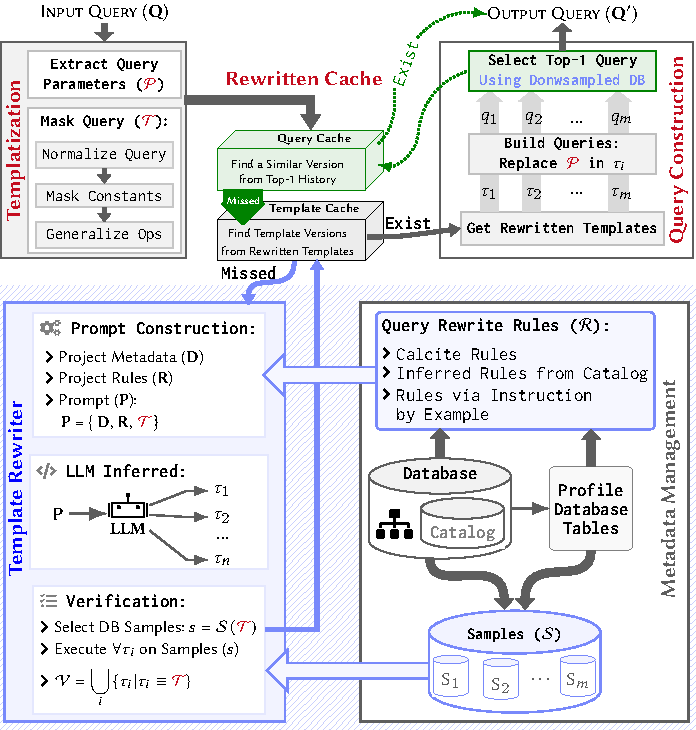
\includegraphics[scale=0.62, keepaspectratio]{fig/fig_ReSequel_Architecture_Slide4.pdf}};
    \node[visible on=<1>] (orig) {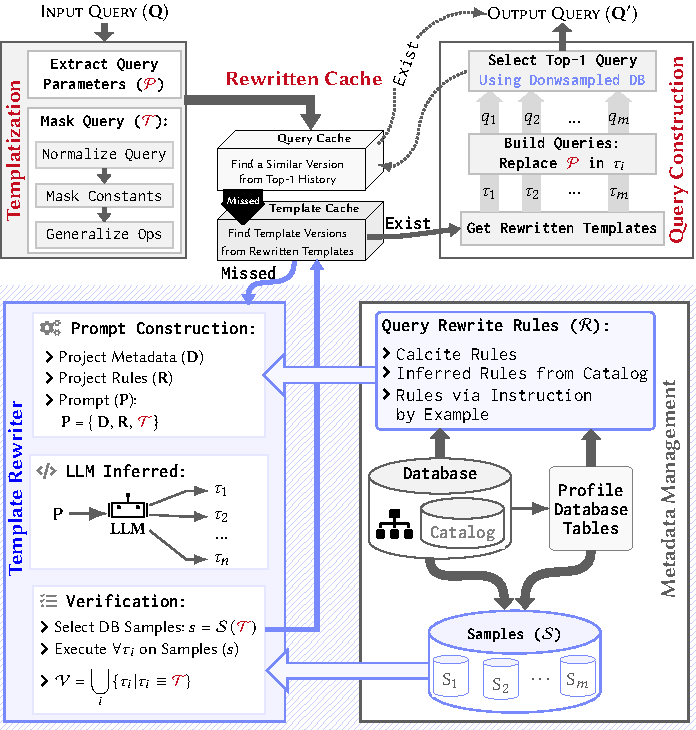
\includegraphics[scale=0.62, keepaspectratio]{fig/fig_ReSequel_Architecture.pdf}};
    \node[visible on=<1>,anchor=north west, text width=0.40\textwidth, align=left,
          font=\scriptsize, inner sep=2pt] (kd) at ($(orig.north east)+(20pt,-40pt)$)
    {%
      \textbf{\textcolor{blue}{Key Design Decisions:}}\\[3pt]
      \setlength\leftmargini{1.2em}%
      \begin{itemize}\setlength\itemsep{1pt}
        \item Outer layer: any DBMS
        \item Template-based: rewrite once
        \item Metadata-guided: schema + stats
        \item Sample-verified: correctness check
        \item Cached: amortized over workload
      \end{itemize}%
    };

    \node[visible on=<2>,anchor=north west, text width=0.40\textwidth, align=left,
          font=\scriptsize, inner sep=2pt] at (kd.north west)
    {%
      \textbf{\textcolor{blue}{Templatization:}}\\[3pt]
      \setlength\leftmargini{1.2em}%
      \begin{itemize}\setlength\itemsep{1pt}
        \item \textbf{Normalize:} canonical form
        \item \textbf{Mask constants:} literals $\rightarrow$ placeholders
        \item \textbf{Generalize ops:} same shape, one key
        \item Output: template \textcolor{tugb}{$\mathcal{T}$} + params \textcolor{tugb}{$\mathbf{P}$}
        \item Effect: many queries, one rewrite
      \end{itemize}%
    };

    \node[visible on=<3>,anchor=north west, text width=0.40\textwidth, align=left,
          font=\scriptsize, inner sep=2pt] (mmtr) at ($(kd.north west)+(0pt,26pt)$)
    {%
      \textbf{\textcolor{blue}{Metadata Management:}}\\[3pt]
      \setlength\leftmargini{1.2em}%
      \begin{itemize}\setlength\itemsep{1pt}
        \item \textbf{Catalog:} schema, keys, constraints
        \item \textbf{Profiling:} per-table/column statistics
        \item \textbf{Rules $\mathcal{R}$:} Calcite, catalog, by-example
        \item \textbf{Samples $\mathcal{S}$:} small, representative
      \end{itemize}%
      \vspace{3pt}
      \textbf{\textcolor{blue}{Template Rewriter:}}\\[3pt]
      \setlength\leftmargini{1.2em}%
      \begin{itemize}\setlength\itemsep{1pt}
        \item \textbf{Prompt $\mathbf{P}$:} metadata + rules
        \item \textbf{LLM proposes} \textcolor{tugb}{$N$} candidate rewrites
        \item Verify on samples, not on full DB
        \item Output: verified set \textcolor{tugb}{$\mathcal{V}$} (\textbf{equivalent only})
      \end{itemize}%
    };

    %% same queries-vs-templates chart as the end-to-end slide, scaled down
    \node[visible on=<3>, anchor=north west, inner sep=1pt, align=left, fill=darkgreen!8]
          at ($(mmtr.south west)+(6pt,-10pt)$)
    {%
      \begin{tikzpicture}[x=0.98mm, y=0.9mm, font=\tiny,
                          bar/.style={draw=black, line width=0.3pt},
                          baseline=(current bounding box.north)]

        %% legend
        \filldraw[bar, fill=black] (0,21.5) rectangle (2.2,23.1);
        \node[right, inner sep=1pt] at (2.2,22.1) {Queries};
        \filldraw[bar, fill=tug]  (11,21.5) rectangle (13.2,23.1);
        \node[right, inner sep=1pt] at (13.2,22.1) {Templates (\# Missed)};

        \foreach \lb/\xx/\nq/\nt in {StackOverflow/1/1190/60, IMDB/21/13646/79} {
          \pgfmathsetmacro{\hq}{4*log10(\nq)}
          %% templates are tiny in comparison -- drop their bars to 30% of the
          %% log height so the contrast with the query bars is visible
          \pgfmathsetmacro{\hgtt}{0.3*2.4*log10(\nt)}
          \pgfmathsetmacro{\xqr}{\xx+4}
          \pgfmathsetmacro{\xtl}{\xx+4.4}
          \pgfmathsetmacro{\xtr}{\xx+8.4}
          \pgfmathsetmacro{\xqc}{\xx+2}
          \pgfmathsetmacro{\xtc}{\xx+6.4}
          \pgfmathsetmacro{\xlc}{\xx+4.2}
          \filldraw[bar, fill=black] (\xx,0)  rectangle (\xqr,\hq);
          \filldraw[bar, fill=tug]   (\xtl,0) rectangle (\xtr,\hgtt);
          \node[above, inner sep=1pt] at (\xqc,\hq) {\nq};
          \node[above, inner sep=1pt] at (\xtc,\hgtt) {\nt};
          \node[below, inner sep=1.5pt] at (\xlc,0) {\textbf{\lb}};
        }
        \draw[gray, line width=0.3pt] (-0.5,0) -- (30,0);
      \end{tikzpicture}%
    };

     \node[visible on=<4>,anchor=north west, text width=0.40\textwidth, align=left,
          font=\scriptsize, inner sep=2pt] at (kd.north west)
    {%
      \textbf{\textcolor{blue}{Query Construction:}}\\[3pt]
      \setlength\leftmargini{1.2em}%
      \begin{itemize}\setlength\itemsep{1pt}
        \item Fetch verified templates $\tau_1,\dots,\tau_m$
        \item \textbf{Bind params:} replace $\mathbf{P}$ in each $\tau_i$
        \item \textbf{Rank candidates} on downsampled DB
        \item \textbf{Select Top-1} query $\mathbf{Q'}$
        \item DBMS executes $\mathbf{Q'}$ unchanged
      \end{itemize}%
    };

     \node[visible on=<5>,anchor=north west, text width=0.40\textwidth, align=left,
          font=\scriptsize, inner sep=2pt] (qc) at ($(kd.north west)+(0pt,22pt)$)
    {%
      \textbf{\textcolor{blue}{Query Cache:}}\\[3pt]
      \setlength\leftmargini{1.2em}%
      \begin{itemize}\setlength\itemsep{1pt}
        \item \textbf{Lookup:} similar query in Top-1 history
        \item \textbf{Hit:} reuse the cached Top-1 rewrite
        \item \textbf{No LLM call}, no sample runs, no ranking
        \item Miss: fall back to the template cache
        \item Cost amortized over the workload
      \end{itemize}%
    };

    %% same chart as overlay 3, plus the query-cache miss series
    \node[visible on=<5>, anchor=north west, inner sep=1pt, align=left, fill=darkgreen!8]
          at ($(qc.south west)+(0pt,-3pt)$)
    {%
      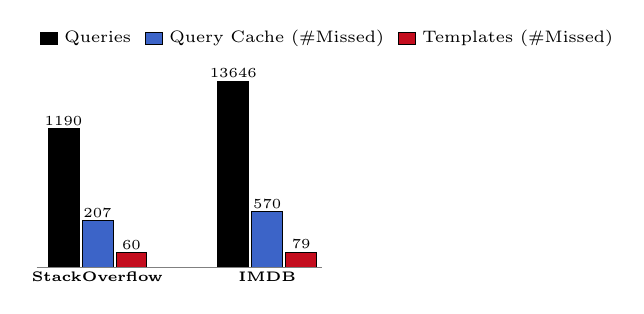
\begin{tikzpicture}[x=0.98mm, y=1.43mm, font=\tiny,
                          bar/.style={draw=black, line width=0.3pt},
                          baseline=(current bounding box.north)]

        %% legend -- one row; each item is chained to the previous one so the
        %% labels can never overlap, whatever their width
        \tikzset{swatch/.style={draw=black, line width=0.3pt, inner sep=0pt,
                                minimum width=2.1mm, minimum height=1.5mm},
                 leg/.style={font=\fontsize{6}{6.5}\selectfont, inner sep=1pt}}
        \node[swatch, fill=black, anchor=west] (sq) at (0,20.3) {};
        \node[leg, right=0.4mm of sq] (lq) {Queries};
        \node[swatch, fill=tugb, right=1.4mm of lq] (sc) {};
        \node[leg, right=0.4mm of sc] (lc) {Query Cache (\#Missed)};
        \node[swatch, fill=tug, right=1.4mm of lc] (st) {};
        \node[leg, right=0.4mm of st] (lt) {Templates (\#Missed)};

        \foreach \lb/\xx/\nq/\nt/\nc in {StackOverflow/1/1190/60/207, IMDB/23/13646/79/570} {
          \pgfmathsetmacro{\hq}{4*log10(\nq)}
          %% templates stay at 30% of the log height; the cache-miss bars are
          %% drawn 2.5x taller so the series is readable next to them
          \pgfmathsetmacro{\hgtt}{0.3*2.4*log10(\nt)}
          \pgfmathsetmacro{\hgtc}{0.75*2.4*log10(\nc)}
          \pgfmathsetmacro{\xqr}{\xx+4}
          \pgfmathsetmacro{\xcl}{\xx+4.4}
          \pgfmathsetmacro{\xcr}{\xx+8.4}
          \pgfmathsetmacro{\xtl}{\xx+8.8}
          \pgfmathsetmacro{\xtr}{\xx+12.8}
          \pgfmathsetmacro{\xqc}{\xx+2}
          \pgfmathsetmacro{\xcc}{\xx+6.4}
          \pgfmathsetmacro{\xtc}{\xx+10.8}
          \pgfmathsetmacro{\xlc}{\xx+6.4}
          \filldraw[bar, fill=black] (\xx,0)  rectangle (\xqr,\hq);
          \filldraw[bar, fill=tugb]  (\xcl,0) rectangle (\xcr,\hgtc);
          \filldraw[bar, fill=tug]   (\xtl,0) rectangle (\xtr,\hgtt);
          \node[above, inner sep=1pt] at (\xqc,\hq) {\nq};
          \node[above, inner sep=1pt] at (\xcc,\hgtc) {\nc};
          \node[above, inner sep=1pt] at (\xtc,\hgtt) {\nt};
          \node[below, inner sep=1.5pt] at (\xlc,0) {\textbf{\lb}};
        }
        \draw[gray, line width=0.3pt] (-0.5,0) -- (36.5,0);
      \end{tikzpicture}%
    };

    %%%%%%%%%%%%%%%%%%%%%%%%%%%%%%%%%%%
    %% progressive build: each step REPLACES the previous one (exact overlay
    %% specs, not <n->), all pinned to orig's north-west so the figure does
    %% not shift between overlays
    \node[visible on=<2>, anchor=north west] (archp1) at (orig.north west)
      {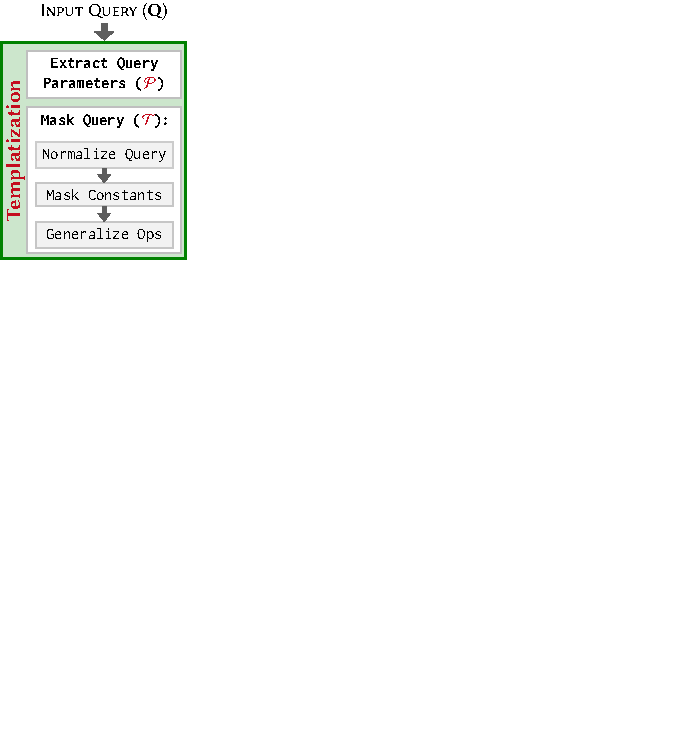
\includegraphics[scale=0.62, keepaspectratio]{fig/fig_ReSequel_Architecture_Slide1.pdf}};
    \node[visible on=<3>, anchor=north west] (archp2) at (orig.north west)
      {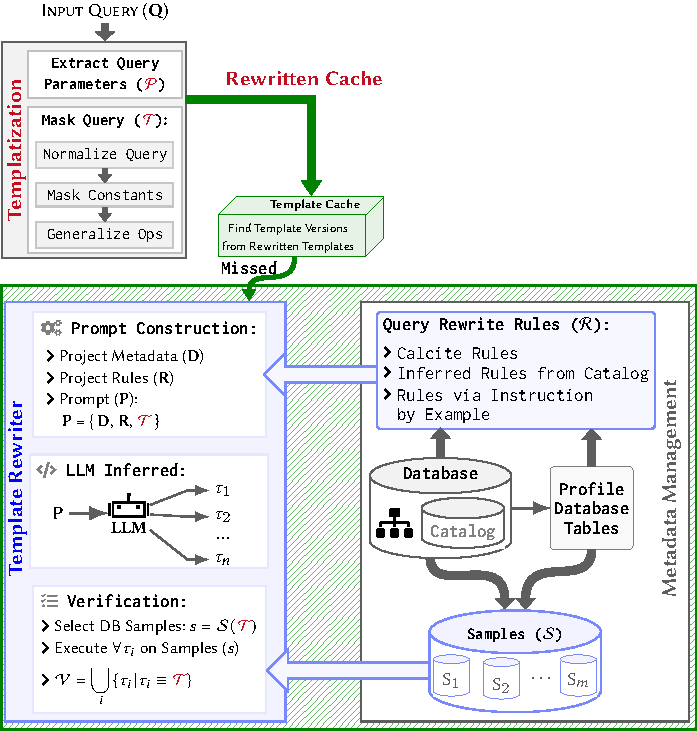
\includegraphics[scale=0.62, keepaspectratio]{fig/fig_ReSequel_Architecture_Slide2.pdf}};
    \node[visible on=<4>, anchor=north west] (archp3) at (orig.north west)
      {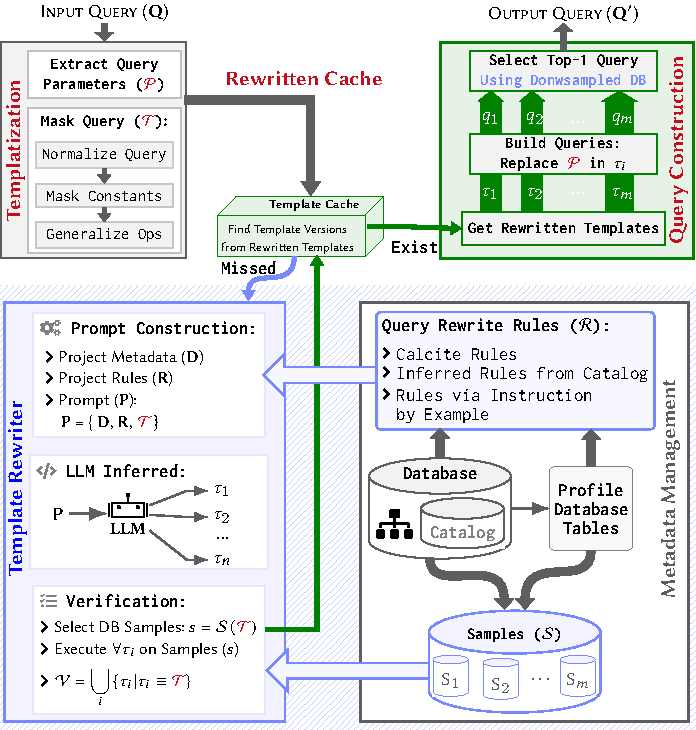
\includegraphics[scale=0.62, keepaspectratio]{fig/fig_ReSequel_Architecture_Slide3.pdf}};
  \end{tikzpicture}
\end{frame}


%% ─── Example 2 ──────────────────────────────────────────────────────
%% Static recap of the motivating example -- all annotations at once
\begin{frame}{\apptitle{tug}{ReSequel}{Recap --- Example 2: Declarative Query Processing}}
  \begin{itemize}
    \item {\footnotesize SQL is \textcolor{tug}{\textbf{declarative}}: the user states \textcolor{blue}{\emph{what}} to compute, the optimizer decides \textcolor{blue}{\emph{how}}.}
  \end{itemize}


\vspace{3mm}
  \scriptsize
  \begin{tikzpicture}
    \node[fill=tugb!5,inner sep=1mm, text=black, xshift=-10pt, line width=0.5pt]  (sql) {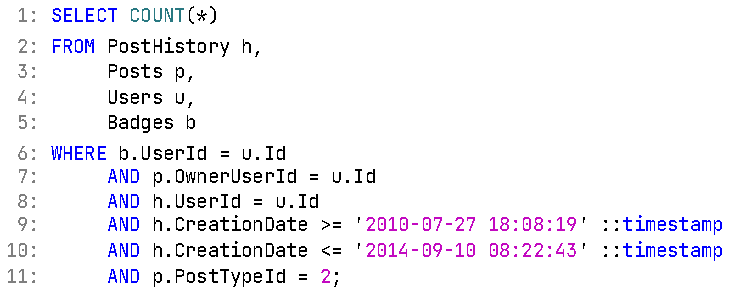
\includegraphics[scale=0.7] {fig/fig_ShowExample_Query_Full.pdf}};

       
    %%%%%%%%%%%%%%%%%%%%%%
    \node [draw=tugb, fill=tugb, line width=0.5pt, minimum width=34pt, minimum height=8pt, fill opacity=0.1] (count1) at($(sql.north west)+(61pt,-8pt)$) {};
     \node[fill=tugb!5, draw=tugb,inner sep=1mm, text=black, line width=0.5pt, right=of count1, xshift=0pt, yshift=0pt]  (pc1) {No early aggregation $\Rightarrow$ huge intermediates};
     \draw[-, tugb, line width=0.5pt, densely dashed]  (count1) -- (pc1);

    %%%%%%%%%%%%%%%%%%%%%%
    \draw[-, tug, line width=0.5pt] ($(sql.north west)+(18pt,-14pt)$) -- ($(sql.north west)+(18pt,-49pt)$) -- ($(sql.north west)+(95pt,-49pt)$) |- ($(sql.north west)+(18pt,-14pt)$);   

    \node[fill=tug!5, draw=tug,inner sep=1mm, text=black, line width=0.5pt, right=of sql, xshift=-130pt, yshift=27pt]  (p1) {Flat 4-way Cross Join};
    \draw[-, tug, line width=0.5pt, densely dashed]  ($(sql.north west)+(95pt,-25pt)$) -- (p1.west);

    %%%%%%%%%%%%%%%%%%%%%%%

    %
    \node [draw=brown, fill=brown, line width=0.5pt, minimum width=34pt, minimum height=8pt,fill opacity=0.1] (u1) at($(sql.north west)+(53pt,-36pt)$) {};
    \node [draw=brown, fill=brown, line width=0.5pt, minimum width=20pt, minimum height=8pt, fill opacity=0.1] (uid1) at($(sql.north west)+(92pt,-55pt)$) {};
    \node [draw=brown, fill=brown, line width=0.5pt, minimum width=20pt, minimum height=8pt, fill opacity=0.1] (uid2) at($(sql.north west)+(122pt,-62.5pt)$) {};
    \node [draw=brown, fill=brown, line width=0.5pt, minimum width=20pt, minimum height=8pt, fill opacity=0.1] (uid3) at($(sql.north west)+(104pt,-71pt)$) {};
   
    \node[fill=brown!5, draw=brown,inner sep=1mm, text=black, line width=0.5pt, right=of sql, xshift=-100pt, yshift=5pt]  (p2) {Join through \textbf{users} is redundant --- it is only a PK bridge};

    \draw[-, brown, line width=0.5pt, densely dashed]  (u1.east) -- (p2.west);
    \draw[-, brown, line width=0.5pt, densely dashed]  (uid1) -- (p2.west);
    \draw[-, brown, line width=0.5pt, densely dashed]  (uid2) -- (p2.west);
    \draw[-, brown, line width=0.5pt, densely dashed]  (uid3) -| (p2.west);


    %%%%%%%%%%%%%%%%%%%%%%%%%%%%%%%%%%%%%%%%%%%%%%%%%%%%%%%%%%%%%
    \node[fill=darkgreen!5, draw=darkgreen,inner sep=1mm, text=black, line width=0.5pt, right=of sql, xshift=-180pt, yshift=-75pt]  (p3) {Filters applied \textbf{after} the join};

    \node [draw=darkgreen,fill=darkgreen!30, line width=0.5pt, minimum width=198pt, minimum height=25pt, fill opacity=0.1] (filter) at($(sql.north west)+(150pt,-88pt)$) {};
    \draw[-, darkgreen, line width=0.5pt, densely dashed]  (filter) -- (p3.north);

    %%%%%%%%%%%%%%%%%%%%%%%%%%%%%%%

    \node[fill=lightgray!30,inner xsep=2mm, inner ysep=1mm, xshift=-10pt, right=of  p3, xshift=40pt, yshift=10pt]  (results) {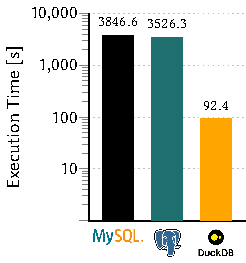
\includegraphics[scale=0.9] {fig/Experiment0-Stats122-baseline.pdf}};
    
  \end{tikzpicture}
\end{frame}

%% ─── SLIDE 15: VERIFICATION ──────────────────────────────────────────────────
\begin{frame}{\apptitle{tug}{ReSequel}{An Example Workflow}}
  \vspace{-2mm}
  \centering
  \begin{tikzpicture}
    %%%%% STEP 1
    \node[fill=none,inner sep=0mm, draw=none]  (sql) {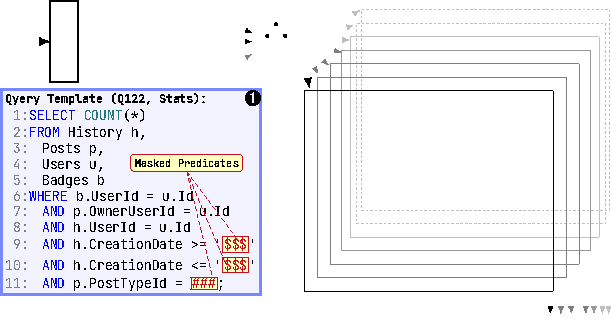
\includegraphics[width=0.78\textwidth, keepaspectratio]{fig/fig_ShowExample_slides_1.pdf}};

    % \pause
    \node[right=of sql, xshift=-20pt, minimum width=80pt, minimum height=0.8\textheight, fill=darkgreen!15] (pipeline) {};

    \node[inner sep=0pt, below=of pipeline.north, yshift=22pt] (pipelinelbl) {\scriptsize \textbf{\textcolor{tug}{Rewriting pipeline:}}};

    \node[below=of pipelinelbl, yshift=20pt, xshift=0pt, fill=white,inner sep=0pt] (pipsql) {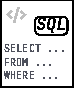
\includegraphics[scale=0.6, keepaspectratio]{fig/fig_SQL.pdf}};

    \node[below=of pipsql, draw=tugb, fill=white, rounded corners=2pt, inner sep=1mm, yshift=10pt] (templatization)
         %% the \ding is \small and the label \tiny; they share a baseline, so the
         %% smaller text reads as sitting low -- raise it onto the icon's optical centre
         {\small\ding{202}\,\raisebox{1.1pt}{\tiny Templatization}};
    
    \draw[-{Latex[scale=0.8]}, line width=1.2pt, black] (pipsql) -- (templatization);     

  
    %%%%% STEP 2
    \node[visible on=<2->, fill=none,inner sep=0mm, draw=none]  (resequel) at(sql) {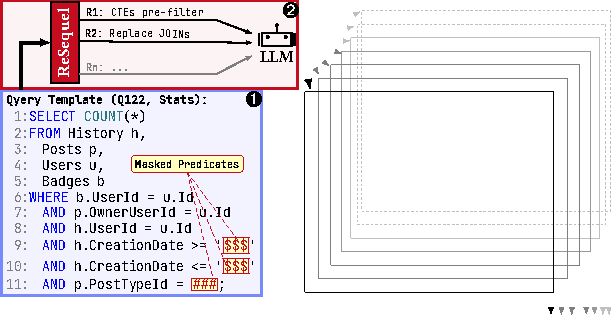
\includegraphics[width=0.78\textwidth, keepaspectratio]{fig/fig_ShowExample_slides_2.pdf}};

    \node[visible on=<2->, below=of templatization, draw=tug, fill=white, rounded corners=2pt,
          inner sep=1mm, yshift=10pt, align=center] (resequelstep)
         {\small\ding{203}\,\raisebox{1.1pt}{\tiny Template Rewriter}\\[-2pt]
          {\tiny \textcolor{gray}{Prompt LLM $\to$ $N$ variants}}};
    
    \draw[visible on=<2->, -{Latex[scale=0.8]}, line width=1.2pt, black] (templatization) -- (resequelstep);    

    %%%%% STEP 3
    \node[visible on=<3->, fill=none,inner sep=0mm, draw=none]  (versions) at(resequel) {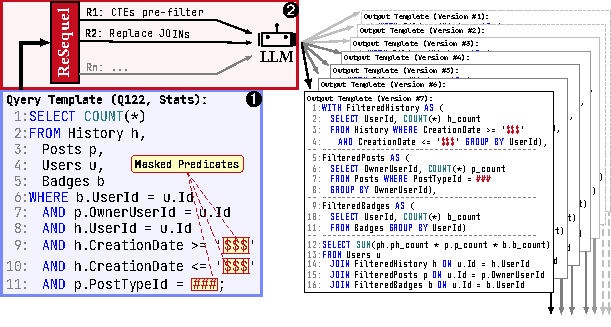
\includegraphics[width=0.78\textwidth, keepaspectratio]{fig/fig_ShowExample_slides_3.pdf}};

    %% align=center is what makes \\ legal inside the node body
    \node[visible on=<3->, draw=darkgreen, fill=none, line width=1.1pt,
          inner sep=2mm, minimum width=50pt, minimum height=25pt, align=center,
          font=\tiny, text=darkgreen] (verify) at ($(resequel.south east)+(-32pt,-7pt)$)
         {Downsample DB (10\%)\\[2pt]
          Verify result equivalence};

    \node[visible on=<3->,  draw=none, fill=white,inner sep=0mm, yshift=10pt] at($(verify.north east)+(-4pt,-13pt)$) {\normalsize\ding{204}}; 
    
    \node[visible on=<3->, below=of resequelstep, draw=darkgreen, fill=white, rounded corners=2pt,
          inner sep=1mm, yshift=10pt, align=center] (verifystep)
         {\small\ding{204}\,\raisebox{1.1pt}{\tiny Verification}};
    
    \draw[visible on=<3->, -{Latex[scale=0.8]}, line width=1.2pt, black] (resequelstep) -- (verifystep);
    
    %%%%% STEP 4

    \node[visible on=<4->, below=of verifystep, draw=gray, fill=white, rounded corners=2pt,
          inner sep=1mm, yshift=10pt, align=center] (top1)
         {\small\ding{205}\,\raisebox{1.1pt}{\tiny Rank $\to$ Cache Top-1}};
    
    \draw[visible on=<4->, -{Latex[scale=0.8]}, line width=1.2pt, black] (verifystep) -- (top1);

    \draw[visible on=<4->, -{Latex[scale=0.9]}, line width=1pt, gray] (verify.west) -- ($(verify.west)+(-37pt,0pt)$);

    \node[visible on=<4->,  draw=none, fill=none,inner sep=0mm, yshift=0pt, left=of verify, yshift=7pt, xshift=20pt] {\normalsize\ding{205}\,\raisebox{1.1pt}{\scriptsize Top-1}}; 

    %% ── runtime of the 10 generated variants, below the figure (left aligned) ──
    %% raw data is in ms, drawn in seconds (value/1000).
    %% Hand-drawn in TikZ so every bar carries its own style; the \foreach
    %% table below is version / seconds / style.
    %% The plot lives in its own picture inside a node: "visible on" is reliable
    %% on a NODE, whereas on a scope (or before a path's own fill) the path
    %% overrides it, and inside a /.style body the overlay spec loops.
    %% anchor=north west puts the picture BELOW the point, whereas the old scope
    %% had its origin there and the bars grew upward -- hence the +36pt lift
    \node[visible on=<4->, anchor=north west, inner sep=0]
         at ($(sql.south west)+(3mm,12pt)$) {%
    \begin{tikzpicture}[fill=lightgray!20,
                  x={0.043\textwidth},         % 10 versions, leaves room for the callout
                  y={0.038\textheight},         % a little taller than before
                  bar/.style={draw=black, line width=0.4pt, rounded corners=1pt},
                  plain/.style={bar, fill=lightgray!10},
                  pick/.style={bar, fill=tug},
                  alt/.style={bar, fill=tugb}]

      %% axes and y ticks (no grid lines)
      \foreach \v in {1,2,3} {
        \draw[gray, line width=0.3pt] (0.32,\v) -- (0.48,\v);
        \node[left, font=\tiny, inner sep=1.5pt] at (0.4,\v) {\v};
      }
      \node[left, font=\tiny, inner sep=1.5pt] at (0.4,0) {0};
      \draw[gray, line width=0.4pt] (0.4,0) -- (0.4,4.1);
      \draw[gray, line width=0.4pt] (0.4,0) -- (10.7,0);

      %% bars -- swap the style name to restyle a single version
      \foreach \i/\v/\st in {1/1.850/plain,  2/3.778/plain, 3/1.624/plain,
                             4/1.604/plain,  5/1.952/plain, 6/1.894/plain,
                             7/1.093/pick,   8/2.173/plain, 9/2.860/plain,
                             10/3.687/alt}
      {
        \filldraw[\st] (\i-0.32,0) rectangle (\i+0.32,\v);
        \node[below, font=\tiny, inner sep=2pt] at (\i,0) {\i};
      }

      %% label the original query inside its bar (10); rotated because the bar
      %% is only ~11pt wide, and white so it reads on the tugb fill
      \node[rotate=90, font=\tiny, text=white] at (9.8,0.5) {orig query};

      %% crown on the selected (Top-1) variant -- bar 7, the fastest one
      \node[above, inner sep=1.5pt, text=color4, font=\scriptsize] at (7,1.093) {\faCrown};

      %% takeaway, parked in the empty band above bars 3--8: the LLM writes ten
      %% plausible rewrites, but only measuring them locally says which to keep
      \node[anchor=north west, align=left, text width=31mm,
            font=\fontsize{5}{5.8}\selectfont,
            fill=white, draw=tug, line width=0.4pt, rounded corners=1.5pt,
            inner xsep=1mm, inner ysep=0.5mm] at (2.7,3.95)
           {\textbf{\textcolor{tug}{LLM proposes, the ReSequel decides}}\\
            valid $\neq$ fast --- timing picks \#7};

      %% axis labels
      \node[below, font=\tiny, inner sep=1pt] at (5.5,-0.75) {\textbf{Versions}};
      \node[rotate=90, anchor=south, font=\tiny, inner sep=1pt]
           at (-0.45,1.8) {\textbf{Time [s]}};
    \end{tikzpicture}};    

    \end{tikzpicture}




%% ── final overlay: dim the workflow and show the end-to-end result ──
\only<5>{%
\begin{tikzpicture}[remember picture, overlay]

  %% frosted-glass wash over the workflow behind
  \fill[white, opacity=0.88]
        (current page.south west) rectangle (current page.north east);

  \node[fill=white, draw=tug, line width=0.8pt, rounded corners=4pt, inner sep=5mm,
        drop shadow={opacity=0.25, shadow xshift=1.5pt, shadow yshift=-1.5pt}]
       at (current page.center) {%
    \begin{minipage}[c]{0.50\textwidth}
      \scriptsize
      \textbf{\textcolor{tug}{What ReSequel did to Q122}}\\[4pt]
      %% ordered by impact: the algebraic win first, then the plan-shape win,
      %% then the input-size win, then the safety/reuse mechanism
      \begin{itemize}\setlength\itemsep{4pt}
        \item \textbf{Factorized join} {\tiny\textcolor{gray}{(eager aggregation)}} ---
              \texttt{COUNT(*)} becomes a \textbf{product of per-key counts};
              the flat join is never materialized
        \item \textbf{No 4-way cross join} --- explicit joins on the CTEs;
              \texttt{Users} was only a PK bridge
        \item \textbf{Filters pushed into the CTEs} --- applied \emph{before} any join
        % \item \textbf{Verified, then cached} --- \textbf{10\%} sample,
        %       \textbf{Top-1} template reused
      \end{itemize}
      \vspace{2mm}
      \centering
      \textcolor{tug}{\textbf{148$\times$--662$\times$ faster, same result}}
    \end{minipage}%
    \hspace{5mm}%
    \begin{minipage}[c]{0.32\textwidth}
      \centering
      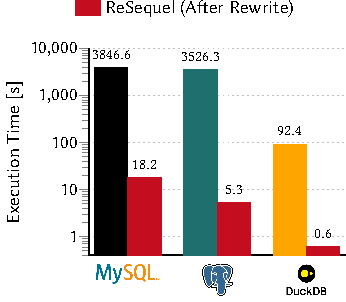
\includegraphics[width=\linewidth]{fig/Experiment0-Stats122-ReSequel.pdf}
    \end{minipage}%
  };
\end{tikzpicture}}

\end{frame}

%% ─── SLIDE 16: OVERALL PERFORMANCE ──────────────────────────────────────────
\begin{frame}{\apptitle{tug}{ReSequel}{End-to-End Performance on Large Workloads}}
\vspace{-2.5mm}
\begin{columns}[T]
\begin{column}{0.75\textwidth}
  \centering
{\setlength{\fboxsep}{3pt}%
\colorbox{tugb!8}{%
 \begin{minipage}{\columnwidth}\centering
 \resizebox{0.75\linewidth}{!}{
\includegraphics{plots/Experiment2-Legend-1-Slide.pdf}}\\[2pt]
   \resizebox{\linewidth}{!}{%
     \begin{tabular}{@{}c@{}}
       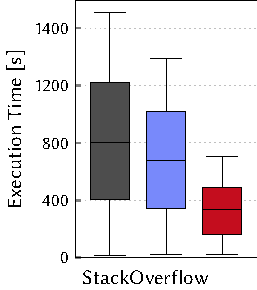
\includegraphics[scale=0.43]{plots/Experiment2-STACKOVERFLOW-PostgreSQL-Slide.pdf}\hspace{0.05cm}%
       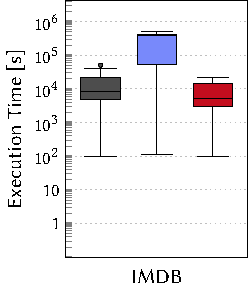
\includegraphics[scale=0.43]{plots/Experiment2-IMDB-PostgreSQL-Slide.pdf}\\[-1pt]
       {\tiny\textbf{\textcolor{tugb}{PostgreSQL}}}
     \end{tabular}%
     %% the rule lives in its own [c]-aligned box so it centres on the plots
     \hspace{1.0mm}%
     \begin{minipage}[c]{0.4pt}\textcolor{tugb}{\rule{0.6pt}{28mm}}\end{minipage}%
     \hspace{1.0mm}%
     \begin{tabular}{@{}c@{}}
       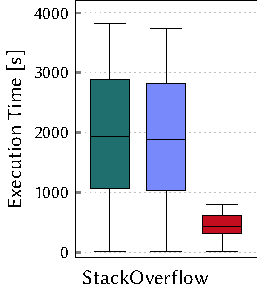
\includegraphics[scale=0.43]{plots/Experiment2-STACKOVERFLOW-MySQL-Slide.pdf}\\[-1pt]
       {\tiny\textbf{\textcolor{tugb}{MySQL}}}
     \end{tabular}%
     \hspace{1.0mm}%
     \begin{minipage}[c]{0.4pt}\textcolor{tugb}{\rule{0.6pt}{28mm}}\end{minipage}%
     \hspace{1.0mm}%
     \begin{tabular}{@{}c@{}}
       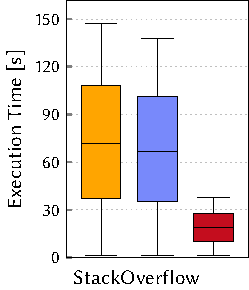
\includegraphics[scale=0.43]{plots/Experiment2-STACKOVERFLOW-DuckDB-Slide.pdf}\hspace{0.05cm}%
       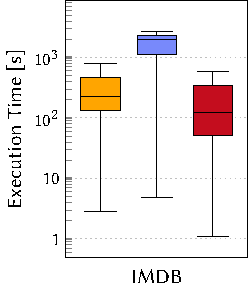
\includegraphics[scale=0.43]{plots/Experiment2-IMDB-DuckDB-Slide.pdf}\\[-1pt]
       {\tiny\textbf{\textcolor{tugb}{DuckDB}}}
     \end{tabular}%
   }
 \end{minipage}}}


  \vspace{3mm}
  {\setlength{\fboxsep}{3pt}%
   \colorbox{lightgray!10}{%
     \begin{minipage}{\columnwidth}\centering    
      % \resizebox{0.5\columnwidth}{!}{%
      %    
\includegraphics{plots/Experiment2-Legend-5ds-Speed.pdf}}\\[2pt]  
       \resizebox{\columnwidth}{!}{%
         %% each plot on its own white panel; the strip behind stays tinted
         \setlength{\fboxsep}{4pt}%
         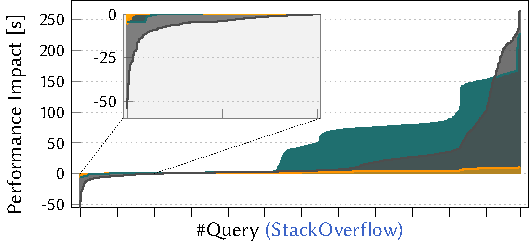
\includegraphics[scale=0.20]{plots/Experiment2-STACKOVERFLOW-Speed-Slide.pdf}\hspace{0.1cm}%
         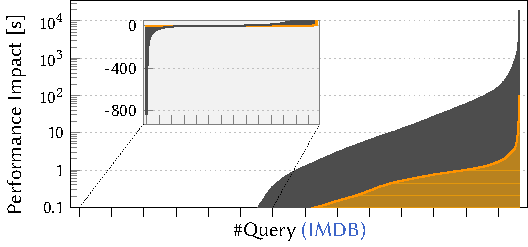
\includegraphics[scale=0.20]{plots/Experiment2-IMDB-Speed-Slide.pdf}%
       }\\[-2pt]
       \begin{minipage}{\columnwidth}\centering
         {\tiny\textbf{\textcolor{tugb}{Individual Performance Impact on Workloads}}}
       \end{minipage}
     \end{minipage}}}

\end{column}

\begin{column}{0.26\textwidth}
  \fontsize{7}{8.4}\selectfont
  \textbf{\textcolor{tug}{Highlights:}}\\[2pt]
  \textbf{Workload speed-up}\\[1pt]
  {\fontsize{6}{7.2}\selectfont
   \setlength{\tabcolsep}{2.5pt}\renewcommand{\arraystretch}{1.25}%
   \begin{tabular}{@{}l c c@{}}
     \rowcolor{tugb!18}
     \textbf{Host DBMS} & \textbf{StackOv.} & \textbf{IMDB}\\
     \rowcolor{tugb!7}
     PostgreSQL & \textcolor{tugb}{\textbf{2.4$\times$}} & \textcolor{tugb}{\textbf{2.3$\times$}}\\
     MySQL      & \textcolor{tugb}{\textbf{4.8$\times$}} & ---\\
     \rowcolor{tugb!7}
     DuckDB     & \textcolor{tugb}{\textbf{3.9$\times$}} & \textcolor{tugb}{\textbf{1.4$\times$}}\\
   \end{tabular}}\\[2mm]
  \setlength{\leftmargini}{1em}%
  \begin{itemize}\fontsize{7}{8.4}\selectfont
    \setlength\itemsep{2pt}\setlength\topsep{0pt}
    \item \textbf{Every host DBMS improves} --- not a single-engine effect\\[1mm]
    \item \textbf{LLM baselines \hred{cannot run}} --- R-Bot, LLM-R2 rewrite
          \emph{per query}\\[1mm]
    \item \textbf{Per query}: most \textcolor{tugb}{speed up}
  \end{itemize}

  \vspace{1mm}
  \centering
  %% queries vs. templates -- log scale, the two counts differ by ~2 orders.
  %% NB: \t, \q are LaTeX accent commands and \ht is a TeX primitive (box
  %% height), so the loop/derived names avoid all three.
  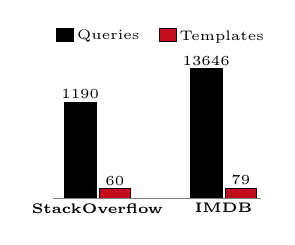
\begin{tikzpicture}[x=1mm, y=1mm, font=\tiny,
                      bar/.style={draw=black, line width=0.3pt}]

    %% legend
    \filldraw[bar, fill=black] (0,20) rectangle (2.2,21.6);
    \node[right, inner sep=1pt] at (2.2,20.6) {Queries};
    \filldraw[bar, fill=tug]  (13,20) rectangle (15.2,21.6);
    \node[right, inner sep=1pt] at (15.2,20.6) {Templates};

    \foreach \lb/\xx/\nq/\nt in {StackOverflow/1/1190/60, IMDB/17/13646/79} {
      \pgfmathsetmacro{\hq}{4*log10(\nq)}
      %% templates are tiny in comparison -- drop their bars to 30% of the
      %% log height so the contrast with the query bars is visible
      \pgfmathsetmacro{\hgtt}{0.3*2.4*log10(\nt)}
      \pgfmathsetmacro{\xqr}{\xx+4}
      \pgfmathsetmacro{\xtl}{\xx+4.4}
      \pgfmathsetmacro{\xtr}{\xx+8.4}
      \pgfmathsetmacro{\xqc}{\xx+2}
      \pgfmathsetmacro{\xtc}{\xx+6.4}
      \pgfmathsetmacro{\xlc}{\xx+4.2}
      \filldraw[bar, fill=black] (\xx,0)  rectangle (\xqr,\hq);
      \filldraw[bar, fill=tug]   (\xtl,0) rectangle (\xtr,\hgtt);
      \node[above, inner sep=1pt] at (\xqc,\hq) {\nq};
      \node[above, inner sep=1pt] at (\xtc,\hgtt) {\nt};
      \node[below, inner sep=1.5pt] at (\xlc,0) {\textbf{\lb}};
    }
    \draw[gray, line width=0.3pt] (-0.5,0) -- (26,0);
  \end{tikzpicture}
\end{column}
\end{columns}
\end{frame}


%% ─── SLIDE 16b: SMALL WORKLOADS (Stats / Stats-CEB) ────────────────────────
\begin{frame}{\apptitle{tug}{ReSequel}{End-to-End Performance on Small Workloads}}
% \vspace{-3mm}
\centering

%% ── row 1: six plots in one line, STATS + STATS-CEB per DBMS ──
{\setlength{\fboxsep}{3pt}%
%% \colorbox builds an \hbox, where \\ is illegal -- the minipage restores a
%% paragraph context for the legend/plot line break
\colorbox{tugb!5}{%
 \begin{minipage}{\linewidth}\centering
   \resizebox{0.7\linewidth}{!}{
\includegraphics{plots/Experiment2-Legend-2-Slide.pdf}}\\[3pt]
   \foreach \dbms [count=\i] in {PostgreSQL, MySQL, DuckDB}{%
     \ifnum\i>1
       \hspace{0.5mm}%
       \begin{minipage}[c]{0.4pt}\textcolor{tugb}{\rule{0.6pt}{30mm}}\end{minipage}%
       %\hspace{1mm}%
     \fi
     \begin{minipage}[c]{0.33\linewidth}\centering
       \includegraphics[scale=0.52]{plots/Experiment2-STATS-\dbms-Slide.pdf}\hspace{0.04cm}%
       \includegraphics[scale=0.52]{plots/Experiment2-STATS-CEB-\dbms-Slide.pdf}\\[0pt]
       {\tiny\textbf{\textcolor{tugb}{\dbms}}}
     \end{minipage}%
   }
 \end{minipage}}}

\vspace{3mm}

%% ── row 2: per-query speedups (left) + highlights (right) ──
\begin{columns}[T]
\begin{column}{0.5\linewidth}
  \centering
  {\setlength{\fboxsep}{3pt}%
   \colorbox{white}{%
     \begin{minipage}{\columnwidth}\centering
      %  \resizebox{0.7\columnwidth}{!}{%
      %    
\includegraphics{plots/Experiment2-Legend-5ds-Speed.pdf}}\\[2pt]
       \resizebox{\columnwidth}{!}{%
         \setlength{\fboxsep}{3pt}%
         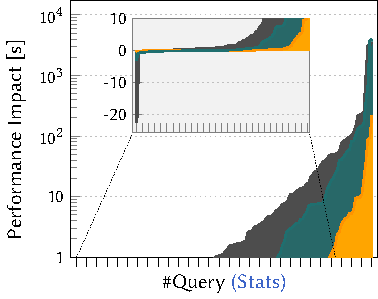
\includegraphics[scale=0.4]{plots/Experiment2-STATS-Speed-Slide.pdf}\hspace{0.3cm}%
         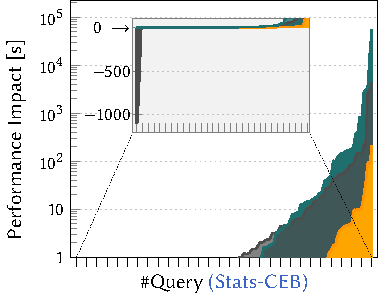
\includegraphics[scale=0.4]{plots/Experiment2-STATS-CEB-Speed-Slide.pdf}%
       }\\[-3pt]
       {\tiny\makebox[0.5\columnwidth]{{\tiny\textbf{\textcolor{tugb}{Individual Performance Impact on Workloads}}}}}
     \end{minipage}
     }}
\end{column}

\begin{column}{0.5\textwidth}
  \fontsize{6.5}{7.8}\selectfont
  \vspace{2mm}
  \textbf{\textcolor{tug}{Highlights:}}\\[3pt]
  \textbf{Workload speed-up:}\\[1pt]
  {\fontsize{6.5}{7.8}\selectfont
   \setlength{\tabcolsep}{7pt}\renewcommand{\arraystretch}{1.15}%
   \begin{tabular}{@{}l c c c@{}}
     \rowcolor{tugb!16}
     \textbf{Workload} & \textbf{PostgreSQL} & \textbf{MySQL} & \textbf{DuckDB}\\
     \rowcolor{tugb!6}
     Stats     & \hblue{5.89$\times$} & \textcolor{gray}{\textbf{1$\times$}} & \hblue{14.85$\times$}\\
     Stats-CEB & \hblue{4$\times$}    & \hblue{3.3$\times$}                 & \hblue{16$\times$}\\
   \end{tabular}}\\[1mm]
  %% \leftmargini is read when the list opens, so shrinking it here pulls the
  %% bullets back to the column edge, flush with the table above.
  \setlength{\leftmargini}{1em}%
  \begin{itemize}\fontsize{6.5}{7.8}\selectfont
    \setlength\itemsep{2pt}\setlength\topsep{0pt}
    \item \textbf{Where the gain comes from}: up to \textbf{20 variants} per query,
          \emph{data}/\emph{catalog} split, redundant \texttt{GROUP BY} removed
    \item \textbf{R-Bot}: rewrites only \textbf{12\%} of the workload --- with
          \hred{negative} impact
    \item \textbf{LearnedRewrite}: per-query, Calcite-bound --- improves few
          queries, \hred{often slowdowns}
  \end{itemize}
\end{column}
\end{columns}
\end{frame}


%%%%%%%%%%%%%%%%%%%%%%%%%%%%%%%%%%%%%%%%%%%%%%%%%%%%%%%%%%%%%%%%%%%%%%%%%%%
%% ════ PART 3: ROLEX ════
%%%%%%%%%%%%%%%%%%%%%%%%%%%%%%%%%%%%%%%%%%%%%%%%%%%%%%%%%%%%%%%%%%%%%%%%%%%
%% Same cover block as CatDB/ReSequel; only title and venue/author differ.
\begin{frame}[plain,noframenumbering]
\begin{tikzpicture}[remember picture, overlay]
  %% ── background: big corner disc + three accent circles ──
  \begin{scope}
    \clip (current page.south west) rectangle (current page.north east);
    \fill[black!58] ($(current page.north east)+(-22mm, 8mm)$) circle (48mm);
    \fill[tugb]     ($(current page.north west)+( 24mm,-22mm)$) circle (13mm);
    \fill[color4]   ($(current page.north west)+( 51mm,-39mm)$) circle (8mm);
    \fill[gray!60]  ($(current page.north west)+( 69mm,-32mm)$) circle (2.5mm);
  \end{scope}

  %% ── full publication title, right-aligned against the rule ──
  \node[anchor=south east, text width=94mm, align=right, inner sep=0, text=black]
    at ($(current page.south west)+(97mm,11mm)$)
    {\large\bfseries \textcolor{darkgreen}{ROLEX:} Workload-optimized Rewrite Rule Discovery and Generation};

  %% ── separator ──
  \draw[black, line width=0.6pt]
    ($(current page.south west)+(101mm,10mm)$) -- ++(0mm,29mm);

  %% ── venue + authors ──
  \node[anchor=north west, text width=48mm, align=left, inner sep=0, text=black]
    at ($(current page.south west)+(106mm,39mm)$)
    {{\normalsize\itshape \textcolor{tugb}{SIGMOD '27}}\\[2pt]
     {\footnotesize\itshape \textcolor{gray}{(under submission)}}\\[8pt]
     {\small\textbf{Saeed Fathollahzadeh}\\[2pt]
      \small Essam Mansour\\[2pt]
      \small Matthias Boehm}};
\end{tikzpicture}
\end{frame}

%% ─── THE OUTER-LAYER STORY (big picture for the whole thesis line) ──────────
\newcommand{\cppfile}[3]{%
  \begin{scope}[shift={(#1,#2)}, line join=round]
    \fill[visible on=<3->, white]
      (-0.45,-0.62) -- (0.45,-0.62) -- (0.45,0.34) -- (0.17,0.62) -- (-0.45,0.62) -- cycle;
    \fill[visible on=<3->, cppblue!15]
      (0.17,0.62) -- (0.17,0.34) -- (0.45,0.34) -- cycle;
    \draw[visible on=<3->, cppblue, line width=0.7pt]
      (-0.45,-0.62) -- (0.45,-0.62) -- (0.45,0.34) -- (0.17,0.62) -- (-0.45,0.62) -- cycle;
    \draw[visible on=<3->, cppblue, line width=0.6pt]
      (0.17,0.62) -- (0.17,0.34) -- (0.45,0.34);
    \node[visible on=<3->, font=\scriptsize, align=center, inner sep=0, text=cppblue!85!black]
      at (0,-0.10) {\texttt{#3}\\[0.4mm]\texttt{.cpp}};
  \end{scope}}

\newcommand{\dbbig}[1]{%
  \makebox[30mm][c]{\includegraphics[height=10mm, width=25mm, keepaspectratio]{fig/logos/#1}}}

\begin{frame}{\apptitle{darkgreen}{ROLEX}{Motivation --- Where Should the LLM Live?}}
\vspace{2mm}
\centering
\resizebox{\linewidth}{!}{%
\begin{tikzpicture}[
  font=\footnotesize,
  layer/.style={rounded corners=3pt, draw, line width=1pt, inner sep=1mm,
                align=center, minimum width=30mm, minimum height=14mm},
  pstep/.style={rounded corners=2.5pt, draw=tugb, fill=white, line width=0.8pt,
                inner sep=1.2mm, align=center, font=\footnotesize,
                minimum width=10mm, minimum height=11mm},
  flow/.style={-{Triangle[width=9pt,length=7pt]}, line width=3pt},
  thin/.style={-{Triangle[width=7pt,length=5.5pt]}, line width=2pt},
  tag/.style={font=\scriptsize\bfseries, inner sep=1pt},
  note/.style={font=\tiny, inner sep=1pt, align=center}]

%% ══ the one thing that never changes: the host engine ═══════════════════
\node[rounded corners=4pt, draw=black!65, fill=white, line width=1.1pt,
      minimum width=25mm, minimum height=85mm, inner sep=1.6mm] (db) at (14.2,-3.8)
     {\shortstack{\textbf{\small{Host DBMS}}\\[0.3mm]{\tiny\textcolor{tug}{(unmodified)}}\\[7mm]
                  \dbbig{postgres.png}\\[5mm]
                  \dbbig{mysql.png}\\[5mm]
                  \dbbig{duckdb.png}}};

%% ══ the measurement, growing one bar series per click ═══════════════════
%% left-aligned in a fixed-width box so the y-axis stays put and the chart
%% extends to the right as ReSequel and then ROLEX are added
\node[anchor=west, inner sep=0, minimum height=54mm] at (17,-3.2)
     {\makebox[88mm][l]{%
        \only<1>{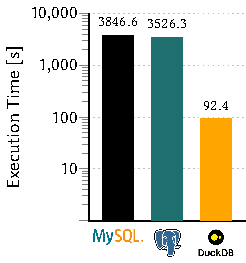
\includegraphics[height=52mm]{fig/Experiment0-Stats122-baseline.pdf}}%
        \only<2>{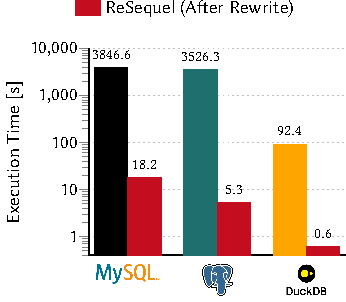
\includegraphics[height=52mm]{fig/Experiment0-Stats122-ReSequel.pdf}}%
        \only<3->{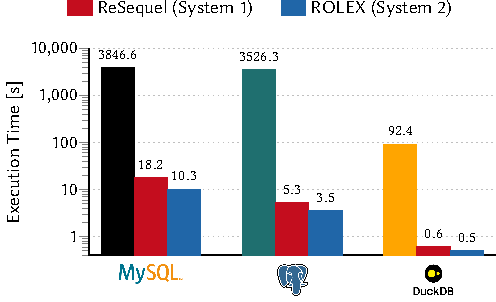
\includegraphics[height=52mm]{fig/Experiment0-Stats122-ReSequelROLEX.pdf}}}};
\node[note, text=gray, anchor=north west] at (17,-6.1)
     {\scriptsize Example~2 --- Stats-CEB query~122};

%% fill=white is essential: the card PDFs are transparent, so without an
%% opaque backing every card in the stack shows through the ones in front
\node[inner sep=0, fill=white]      at (1.22,-0.345) {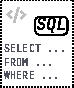
\includegraphics[height=20mm]{fig/fig_SQLDot.pdf}};
\node[inner sep=0, fill=white]      at (1.02,-0.215) {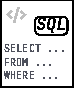
\includegraphics[height=20mm]{fig/fig_SQL.pdf}};
\node[inner sep=0, fill=white]      at (0.82,-0.085) {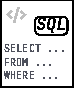
\includegraphics[height=20mm]{fig/fig_SQL.pdf}};
\node[inner sep=0, fill=white] (q1) at (0.62, 0.045) {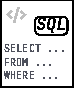
\includegraphics[height=20mm]{fig/fig_SQL.pdf}};
\draw[flow, black!60] (2.25,-0.15) -- (12.5,-0.15);

%% ══ row 2 -- ReSequel hangs off the same query rail ═════════════════════
\node[visible on=<2->, layer, draw=tug, fill=white] (l2) at (6.3,-2.00)
     {\textbf{\textcolor{tug}{\small{ReSequel}}}\\[1.2mm]
      \only<2->{
\includegraphics[height=6mm]{fig/logos/openai.pdf}\hspace{1.8mm}%
      
\includegraphics[height=6mm]{fig/logos/gemini.pdf}\hspace{1.8mm}%
      
\includegraphics[height=6mm]{fig/logos/meta.pdf}}};
\draw[visible on=<2->, flow, tug, rounded corners=5pt] ($(q1.south)+(20pt,-13pt)$) |- (l2);
\draw[visible on=<2->, flow, tug] (l2) -- (db.west|-l2);

%% ReSequel's limitations, as a callout balloon pointing at the box itself
%% (same idiom as the CatDB motivation slide)
\node[visible on=<2->, rectangle callout, rounded corners=2pt,
      callout absolute pointer={($(l2.north) +(0pt,0pt)$)},
      callout pointer width=8pt,
      fill=tug!5, draw=tug, line width=0.6pt, text=black, inner sep=1.6mm,
      anchor=west, text width=65mm, font=\footnotesize, align=left] at (5.2,1.6)
     {\textcolor{tug}{\textbf{Today --- the query is executed \emph{as written}}}\\[1.5mm]
      \textcolor{tug}{\ding{56}}\ One LLM call \textbf{per template} ---
        \$, latency, non-determinism\\[1mm]
      \textcolor{tug}{\ding{56}}\ Free-form SQL --- the insight is
        \textbf{thrown away} after the query\\[1mm]
      \textcolor{tug}{\ding{56}}\ Verified \textbf{per query} on samples};

\node[visible on=<4->, rounded corners=2pt, draw=tugb, line width=1pt,
      pattern=north east lines, pattern color=tugb!10,
      minimum width=89.5mm, minimum height=67mm] (rolexbox) at (7.3,-6.2) {};

\node[visible on=<4->, draw=none,text=tugb,font=\normalsize\bfseries, below=of rolexbox.south, yshift=20pt] {ROLEX};      
%% ── first, above: the offline loop that BUILDS the rules ───────────────
%% the (Q,Q'') pair produced by row 2 is the raw material
\draw[visible on=<4->, densely dashed, line width=1.1pt, tugb]
      (3,-2.00) -- (3,-3.60) -- (9.5,-3.60) -- (9.5,-2.00);
% \draw[visible on=<4->, thin, gray] (2.2,-3.60) -- (2.2,-4.00);
\node[visible on=<4->, note, fill=white, inner sep=0.8mm, anchor=south] (selectqqq) at (6.2,-3.58)
     {\scriptsize $(Q,\,Q'')$ pairs from the sampled workload};

\node[visible on=<4->, pstep, inner sep=0, draw=none, fill=none, font=\small\bfseries] (q) at (3,-1.75) {$Q$};
 \node[visible on=<4->, pstep, inner sep=0, draw=none, fill=none, font=\small\bfseries] (q) at (9.5,-1.75) {$Q''$};    

%% the two IR plans with a delta between them: exactly what Distill computes
\node[visible on=<4->, pstep, fill=tugb!4] (dis) at (4,-5)
     {\textbf{Distill}\\[2mm]
      \only<4->{
\includegraphics[height=5mm]{fig/fig_AST.pdf}}\;{\scriptsize$\Delta$}\;%
      \only<4->{
\includegraphics[height=5mm]{fig/fig_ASTFK.pdf}}};
\node[visible on=<4->, pstep, fill=tugb!4] (imp) at (6,-5)
     {\textbf{Implement}\\[0.3mm]{\tiny C++ rule}\\[0.5mm]
      \only<4->{
\includegraphics[height=3mm]{fig/logos/openai.pdf}\hspace{1.0mm}%
      
\includegraphics[height=3mm]{fig/logos/gemini.pdf}\hspace{1.0mm}%
      
\includegraphics[height=3mm]{fig/logos/meta.pdf}}};
\node[visible on=<4->, pstep, draw=tugb, fill=tugb!4] (ver) at (8.50,-5)
     {\textbf{Verify}\\[0.3mm]{\tiny Smoke$/$SMT $/$ Sample}};

\draw[visible on=<4->, thin, tugb] (dis) -- (imp);
\draw[visible on=<4->, thin, tugb] (imp) -- (ver);
\draw[visible on=<4->, thin, tugb, rounded corners=4pt] (selectqqq.south) -- ($(selectqqq.south)+(0pt,-3mm)$) -| (dis.north);


%% ── then, below: the artifact those rules land in, and the online path ─
\node[visible on=<3->, rounded corners=3pt, draw=tugb, fill=tugb!4, line width=1pt,
      minimum width=65mm, minimum height=30mm] (rw) at (6.5,-7.7) {};
\node[visible on=<3->, font=\small\bfseries, text=tugb, anchor=north]
     at (6.45,-6.28) {\texttt{\textbf{Rewriter.cpp}}};
\node[visible on=<3->, inner sep=0] at (4.35,-7.28) {\only<3->{
\includegraphics[height=8mm]{fig/fig_Index.pdf}}};
\node[visible on=<3->, font=\scriptsize, text=black, anchor=north] at (4.25,-7.75) {Rule Index};
\cppfile{5.75}{-7.55}{Rule1}
\cppfile{6.95}{-7.55}{Rule2}
\node[visible on=<3->, font=\small, text=tugb] at (7.85,-7.45) {$\cdots$};
\cppfile{8.8}{-7.55}{RuleN}

\draw[visible on=<3->, flow, tugb, rounded corners=5pt] ($(q1.south)+(0pt,-13pt)$) |- (rw);
\draw[visible on=<3->, flow, tugb] (rw) -- (db.west|-rw);
\draw[visible on=<4->, thin, tugb, rounded corners=4pt] (ver.south) -- (ver.south|-rw.north) ;
\node[visible on=<4->, note, text=color4!70!black, anchor=west] at (8.60,-5.85) {\scriptsize registered as \texttt{RuleN.cpp}};

\node[visible on=<3->, fill=white, inner sep=1.1mm] (nollm) at (6.95,-8.70)
     {\only<3->{
\includegraphics[height=3.6mm]{fig/logos/openai.pdf}\hspace{1.4mm}%
      
\includegraphics[height=3.6mm]{fig/logos/gemini.pdf}\hspace{1.4mm}%
      
\includegraphics[height=3.6mm]{fig/logos/meta.pdf}}};

\draw[visible on=<3->, tug, line width=1.1pt, rounded corners=1.5pt]
      (nollm.south west) rectangle (nollm.north east);
\draw[visible on=<3->, tug, line width=1.1pt]
      (nollm.south west) -- (nollm.north east);

%% ── what the move buys: parked bottom-right and wired back to the ROLEX
%% zone, so it reads as a consequence of that box rather than a floating list
\node[visible on=<4->, rectangle callout, rounded corners=2pt,
      callout absolute pointer={($(rolexbox.east)+(0pt,-2.6cm)$)},
      callout pointer width=8pt,
      fill=darkgreen!5, draw=darkgreen, line width=0.6pt, text=black, inner sep=1.6mm,
      anchor=north west, text width=65mm, font=\footnotesize, align=left] (ben) at (16.1,-7.80)
     {\textcolor{darkgreen}{\textbf{With ROLEX --- rules}}\\[1.5mm]
      \textcolor{darkgreen}{\ding{52}}\ \textbf{Reproducible} --- same rewrite every run\\[1mm]
      \textcolor{darkgreen}{\ding{52}}\ \textbf{Reusable} --- one rule, many queries\\[1mm]
      \textcolor{darkgreen}{\ding{52}}\ \textbf{Cheap} --- zero online LLM cost\\[1mm]
      \textcolor{darkgreen}{\ding{52}}\ \textbf{Verified} --- Smoke $/$ SMT $/$ sample, once};

\end{tikzpicture}}
\end{frame}


%% ─── ROLEX EXPERIMENT 1: OFFLINE RULE-GENERATION COST ────────────────────────
%% Both plots come straight from the ROLEX paper (Figure exp0): the elapsed-time
%% breakdown (Distill/Generate/Verify vs. the baselines) and the token budget.
\begin{frame}{\apptitle{darkgreen}{ROLEX}{What the Rules Cost to Build --- Paid Once, Offline}}
\vspace{-1.5mm}
\centering
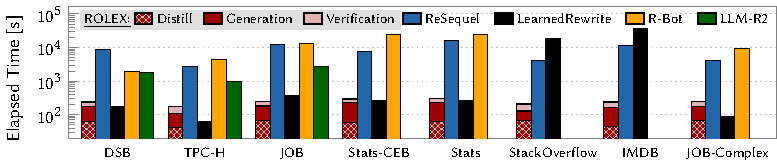
\includegraphics[width=0.80\linewidth]{plots/Experiment0-Quantization.pdf}\\[-1mm]
{\scriptsize\textcolor{tugb}{(a) Rule-generation time per workload ---
 the baselines pay their cost \emph{per query}, at runtime}}

\vspace{1.5mm}
\begin{columns}[T]
\begin{column}{0.40\textwidth}
  \centering
  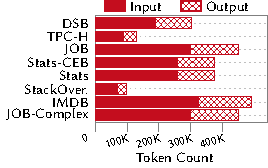
\includegraphics[width=0.95\linewidth]{plots/Experiment0-Tokens.pdf}\\[0.5pt]
  {\scriptsize\textcolor{tugb}{(b) LLM tokens per workload}}
\end{column}
\begin{column}{0.6\textwidth}
  \fontsize{7.2}{8.6}\selectfont
  \textbf{\textcolor{tug}{Highlights:}}\\[1pt]
  \begin{itemize}\setlength\itemsep{1.8pt}\setlength\topsep{0pt}\setlength\parskip{0pt}
    \item \textbf{Paid once, then free} --- \textcolor{tugb}{$\sim$2--5\,$\times$10$^2$\,s} per workload;
          R-Bot and LLM-R2 call the LLM \hred{for every query}\\[2mm]
    \item \textbf{Distill $\to$ Generate $\to$ Verify}, all in memory ---
          the cost is \textbf{DBMS-independent}\\[2mm]
    \item \textbf{118 rules $\to$ \textcolor{tugb}{60 distinct}} after cross-workload dedup;
          tokens track only the \emph{new} rules\\[2mm]
    % \item \textbf{ReSequel's templates do not scale}: 60 cover
    %       \hred{1{,}190 of 18{,}251} StackOverflow queries
    \item \textbf{LLM-R2} also needs \hred{per-workload re-training}
  \end{itemize}
\end{column}
\end{columns}
\end{frame}

%% ─── ROLEX EXPERIMENT 2: AGAINST A BESPOKE QUERY COMPILER ────────────────────
%% SynnoDB (formerly BespokeOLAP) compiles each query to native code over Parquet;
%% the plot separates its I/O + ingest + preprocessing from actual query time.
\begin{frame}{\apptitle{darkgreen}{ROLEX}{vs.\ a SynnoDB (BespokeOLAP) Query Compiler --- CEB Workload at Scale}}
\vspace{-2mm}
\centering
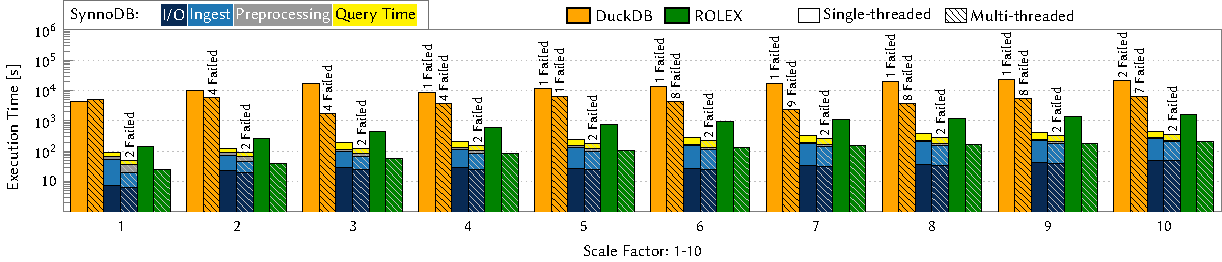
\includegraphics[width=\linewidth]{plots/Experiment0-Micro-CEB.pdf}\\[-1mm]
{\scriptsize\textcolor{tugb}{16 CEB queries over IMDB, SF\,1--10 --- \textsf{SynnoDB}
 compiles each query to native code over Parquet}}

\vspace{1.5mm}
{\fontsize{7.2}{8.6}\selectfont
\begin{columns}[T]
\begin{column}{0.485\textwidth}
  \textbf{\textcolor{blue}{Why ROLEX wins:}}\\[1pt]
  \begin{itemize}\setlength\itemsep{1.8pt}\setlength\topsep{0pt}\setlength\parskip{0pt}
    \item Attacks the \textbf{asymptotic cause}: factorized \texttt{COUNT(*)} keeps
          intermediates \textcolor{tugb}{under 50\,GB} --- nothing spills
    \item 4 queries are \textbf{93\%} of DuckDB's time $\to$
          \textcolor{tugb}{378$\times$, 220$\times$, 102$\times$, 34$\times$};
          32 threads now \emph{help} (\textcolor{tugb}{5.5--7.8$\times$})
    \item \textbf{All 16 complete}, every SF --- end-to-end
          \textcolor{tugb}{1.97$\times$}/\textcolor{tugb}{1.81$\times$} over SynnoDB
  \end{itemize}
\end{column}
\begin{column}{0.485\textwidth}
  \textbf{\textcolor{tug}{Where the baselines break:}}\\[1pt]
  \begin{itemize}\setlength\itemsep{1.8pt}\setlength\topsep{0pt}\setlength\parskip{0pt}
    \item \textbf{SynnoDB} executes fastest --- but I/O $+$ ingest $+$ preprocessing
          are \hred{58--77\%} of wall clock
    \item \textbf{SynnoDB} multi-threaded \hred{crashes} (\texttt{SIGSEGV}) on 11a/11b
          at \emph{every} scale factor
    \item \textbf{DuckDB} spills $\sim$800\,GB against 148\,GB RAM: 32 threads are
          \hred{slower than 1}, 4--9 queries time out
  \end{itemize}
\end{column}
\end{columns}}
\end{frame}



%% ─── SUMMARY ────────────────────────────────────────────────────────────────
%% Closes the arc: the same recipe instantiated three times, with the grounding
%% signal and the verification mechanism named explicitly for each system.
%% The tabular is wrapped in \resizebox so the last column can never overflow.
\begin{frame}{\apptitle{black!60}{Conclusion}{Summary and Lessons Learned}}
\vspace{5mm}
\begin{exampleblock}{}
  \centering\small
  \textbf{One recipe, three systems:} generate with an LLM, \hgreen{verify with the system},
  keep only what is \textbf{correct} and \textbf{fast}
\end{exampleblock}

\vspace{2mm}
\centering
\resizebox{\linewidth}{!}{%
\fontsize{7.6}{9.4}\selectfont
\setlength{\tabcolsep}{5pt}%
\renewcommand{\arraystretch}{1.35}%
\begin{tabular}{@{}l l l l@{}}
\toprule
\textbf{System} & \textbf{What grounds the LLM} & \textbf{What verifies it} & \textbf{Headline result} \\
\midrule
\textcolor{tugb}{\textbf{CatDB}} & data catalog $+$ refined schema
  & execute \& auto-repair
  & \textcolor{tugb}{up to 52\% accuracy} \\
\textcolor{tug}{\textbf{ReSequel}} & query templates $+$ metadata
  & sample-based equivalence
  & \textcolor{tug}{2.5--16$\times$} per workload \\
\textcolor{darkgreen}{\textbf{ROLEX}} & the \emph{workload} itself
  & SMT $+$ sample, once, offline
  & \textcolor{darkgreen}{60\%} below ReSequel, \hgreen{zero} LLM online \\
\bottomrule
\end{tabular}}

\vspace{3mm}
\raggedright
{\scriptsize
\textbf{\textcolor{tug}{Lessons learned:}}\\[2pt]
\begin{itemize}\setlength\itemsep{2.5pt}\setlength\topsep{0pt}
  \item \textbf{Show the model the real data} --- the catalog, the schema, the
        real queries; it cannot guess them
  \item \textbf{Always check the answer} --- a pipeline or a rewrite that looks
        right can still be wrong
  \item \textbf{Ask the LLM once, not per query} --- keep what it found, and every
        later query is free
\end{itemize}}

\only<2->{%
\begin{tikzpicture}[remember picture, overlay]
  \node[rotate=30, anchor=east, text=tug, font=\large\bfseries]
       at ($(current page.north east)+(-16mm,-6mm)$) {Thank You!};
\end{tikzpicture}}
\end{frame}


% ════ ACKNOWLEDGEMENTS ════
%% Braced like the appendix block, so the footer override below stays local.
{%
%% Same footer bar as the main deck, minus the "n / 25" counter: like the
%% appendix, these closing slides sit outside that count -- printing it here
%% used to read as 26/25.
\setbeamertemplate{footline}{%
    \leavevmode%
    \usebeamerfont{footline}%
    \hbox{%
        \begin{beamercolorbox}[wd=.65\textwidth, ht=3ex, dp=1.25ex,
            left, leftskip=2em]{footline}%
            \insertshorttitle%
        \end{beamercolorbox}%
        \begin{beamercolorbox}[wd=.35\textwidth, ht=3ex, dp=1.25ex,
            right, rightskip=4em]{footline}%
            \insertshortauthor\hspace{1em}Acknowledgements%
        \end{beamercolorbox}%
    }%
}

%% ─── ACKNOWLEDGEMENTS: SECTION DIVIDER ───────────────────────────────────────
%% Plain full-bleed slide, single centred word.  Reuses the corner-disc motif of
%% the paper cover slides so the deck reads as one piece.
\begin{frame}[plain,noframenumbering]
\begin{tikzpicture}[remember picture, overlay]
  \begin{scope}
    \clip (current page.south west) rectangle (current page.north east);
    \fill[black!58] ($(current page.north east)+(-22mm, 8mm)$) circle (48mm);
    %% accent circles pulled higher than on the cover slides: there the title
    %% sits at the bottom, here it runs straight through the page centre.
    \fill[tugb]     ($(current page.north west)+( 24mm,-19mm)$) circle (13mm);
    \fill[color4]   ($(current page.north west)+( 51mm,-26mm)$) circle (8mm);
    \fill[gray!60]  ($(current page.north west)+( 69mm,-19mm)$) circle (2.5mm);
  \end{scope}

  \node[inner sep=0, text=tug, font=\Huge\bfseries] (ack)
    at (current page.center) {ACKNOWLEDGEMENTS};
  \draw[tug, line width=0.8pt]
    ([yshift=-5mm]ack.south west) -- ([yshift=-5mm]ack.south east);
\end{tikzpicture}
\end{frame}

%% ─── ACKNOWLEDGEMENTS ────────────────────────────────────────────────────────
%% Photo row with two-line names underneath, in the style of the sample deck.
%% \memberpic is defined outside the frame: beamer re-reads frame bodies, where
%% a bare #1 is illegal.  NB Juergen's portrait ships as .webp, which xelatex
%% cannot read -- it was converted to .png alongside the original.
\newcommand{\memberpic}[3]{%
  \begin{minipage}[t]{0.235\textwidth}\centering
    \setlength{\fboxsep}{0pt}%
    \fcolorbox{black!25}{white}{\includegraphics[width=30mm]{fig/members/#1}}\\[3mm]
    {\normalsize #2\\[1pt] #3}
  \end{minipage}}

\begin{frame}[noframenumbering]{Acknowledgements}
\vspace{1mm}
{\large Thank you to my committee members!}

\vspace{8mm}
\centering
\memberpic{Carsten-Binnig-sq.jpg}{Carsten}{Binnig}\hfill
\memberpic{Juergen-Rilling.png}{Juergen}{Rilling}\hfill
\memberpic{Abdelhak-Bentaleb.jpg}{Abdelhak}{Bentaleb}\hfill
\memberpic{Jun-Yan.jpeg}{Jun}{Yan}
\end{frame}

%% ─── ACKNOWLEDGEMENTS: SUPERVISORS ───────────────────────────────────────────
%% Message left, portraits right -- the layout of the sample deck's advisor
%% slide.  Each portrait carries the date the supervision started.


\newcommand{\supervisorpic}[3]{%
  \begin{minipage}[t]{0.47\linewidth}\centering
    \setlength{\fboxsep}{0pt}%
    \fcolorbox{black!25}{white}{\includegraphics[width=33mm]{fig/members/#1}}\\[3mm]
    {\normalsize #2}\\[1.5mm]
    {\footnotesize\textcolor{gray}{#3}}
  \end{minipage}}

\begin{frame}[noframenumbering]{Acknowledgements}
\vspace{3mm}
\begin{columns}[c]
\begin{column}{0.39\textwidth}
  {\large Thank you \textbf{Essam} and \textbf{Matthias}\\[2mm]
for teaching me to ask better questions --- and trusting me to answer them
my own way.}
\end{column}
\hfill
\begin{column}{0.57\textwidth}
  \centering
  \supervisorpic{essam_3.jpg}{Essam Mansour}{Since September 2023}\hfill
  \supervisorpic{MatthiasBoehm.jpg}{Matthias Boehm}{Since April 2021}  
\end{column}
\end{columns}
\end{frame}
}

\end{document}
